%%%%%%%%%%%%%%%%%%%%%%%%%%%%%%%%%%%%%%%%%%%%%%%%%%%%%%%%%%%%%%%%%%%%%%
% You must use the Makefile to build this document ... it includes
% the proper documentclass here.  The available document classes are
% standard_dc.tex
% handout_dc.tex
%%%%%%%%%%%%%%%%%%%%%%%%%%%%%%%%%%%%%%%%%%%%%%%%%%%%%%%%%%%%%%%%%%%%%%

%%%%%%%%%%%%%%%%%%%%%%%%%%%%%%%%%%%%%%%%%%%%%%%%%%%%%%%%%%%%%%%%%%%%%%
%% Abstract
%% 
%% LibMesh is an open-source finite element library that was originally
%% developed to facilitate serial and parallel simulation of multiscale,
%% multiphysics applications using adaptive mesh refinement and
%% coarsening strategies.  The library was created in the CFDLab at the
%% University of Texas's Aerospace Engineering and Engineering Mechanics
%% Department, but, as with other open-source software projects,
%% contributions are being made elsewhere in the US and abroad.  In this
%% talk, which will be geared toward a general audience, we will describe
%% the underlying philosophy and software design approach used in the
%% library.  We will give additional details on the adaptive mesh
%% refinement and coarsening (AMR/C) schemes utilized, and finally,
%% describe our implementations in the key areas of domain decomposition,
%% message passing, and parallel mesh data structures.  Other topics
%% include: discussion of C++ programming paradigms (scientific software
%% and the STL) software reusability in the face of diverse user
%% applications, and integration with high-level threading APIs for
%% making efficient use of hybrid parallel architectures.  Finally,
%% results from some of the various applications which utilize the
%% library are presented, and areas of future research are discussed.
%%%%%%%%%%%%%%%%%%%%%%%%%%%%%%%%%%%%%%%%%%%%%%%%%%%%%%%%%%%%%%%%%%%%%%


% Everything before \begin{document}
%%%%%%%%%%%%%%%%%%%%%%%%%%%
% LaTeX package inclusion %
%%%%%%%%%%%%%%%%%%%%%%%%%%%
\usepackage{times}
\usepackage{units}
\usepackage{mathrsfs}
% \usepackage{diss} % defines \bv and some other stuff
\usepackage{subfigure}
\usepackage{multirow}
\usepackage{amsmath}
\usepackage{amssymb}
%\usepackage{movie15} % Do not use w/ multimedia
\usepackage{multimedia}
\usepackage{algorithm}
\usepackage{algorithmic}
%\usepackage{verbatim} % DO NOT include verbatim.  I think it messes up the semiverbatim environment!
\usepackage{booktabs}

% Package to include when making a handout.  You will probably need to install
% PGF before you can use these.  I did not yet find an RPM :-(
% Something seems to be wrong with this package.  It gives me a bunch of the following errors:
% Illegal unit of measure (pt inserted).
%\usepackage{pgf,pgfpages}
%\pgfpagesuselayout{4 on 1}[letterpaper,landscape,border shrink=0.5in]




% makes slide bg slightly gray in handouts, may help delineate slide boundaries
% Note that you can make acrobat print slide borders automatically as well...
%\mode<handout>{\setbeamercolor{background canvas}{bg=black!5}} 
\setlength{\fboxrule}{1pt} % Thicker boxes may help you in setting viewports
\setlength{\fboxsep}{0pt} % amt of space between the rule and the contents of the box.


%\usepackage{optional}
%\usepackage[
%bookmarks=true,
%colorlinks=true,
%linkcolor=black,
%filecolor=blue,
%pagecolor=black,
%urlcolor=black]{hyperref}


\usepackage{hyperref}
\usepackage{multimedia}

% Subfig is a replacement for subfigure.  It defines subfloat environment.
% DOES NOT WORK WITH BEAMER
%%\usepackage{subfig} 
%% \captionsetup[subfloat] % This option applies to all *subfloats*
%%              {
%%                %labelformat=empty % Do not put (a), (b), etc. in subfigure captions
%%                %,listofformat=subparens
%%                farskip=5pt
%%              } 



%\usetheme{Darmstadt} % progress bubbles and subsection headers
%\usetheme{Frankfurt} % progress bubbles no  subsection headers
%\usetheme{Goettingen} % Triangle bullets, Right-navigation bar,
                       % can screw up long titles and absolute-spaced images!
                       % top-aligned slides can end up looking wrong.
%\usetheme{Hannover}   % Goettingen with nav bar on left
\usetheme{Antibes}     % Square bullets, top nav section+subsection Windows explorer
                       % drop-down navigation

% You can apparently combine multiple color themes.
%\usecolortheme{sidebartab}% special - changes colors in sidebar s.t. current entry is highlighted

%\usecolortheme{lily} % UNinstall block colors from another theme


% ``Complete'' color themes completely specify all colors and have
% names of flying animals
%\usecolortheme{albatross} % blue background!
%\usecolortheme{beetle} % (dark) gray background
\mode<handout>{\usecolortheme{dove}} % white almost everywhere: good for printing or handout!
%\mode<handout>{\usecolortheme{seagull}} % like dove but with shades of gray allowed

% ``Inner'' color themes only specify the colors of elements used in inner themes
% Can be used together with other color themes, have names of flowers.
\mode<beamer>{\usecolortheme{orchid}} % white on dark block titles.  use w/ whale.
%\usecolortheme{rose} % more subdued color combination than orchid.  about right with seahorse?


% ``Outer'' color themes.  Change the palette colors for headline,
% footline, and sideline.  Sea creature names.
\mode<beamer>{\usecolortheme{whale}} % darkest top titles, usually used by CFDLab presenters
%\usecolortheme{dolphin} % was used by Ben in his diss.  b/w whale and seahorse contrast-wise.
%\usecolortheme{seahorse}

% Force any theme (eg Antibes) to use circle bullets
% \setbeamertemplate{itemize items}[circle]

% Use an arbitrary symbol (double right arrow) for an itemize bullet
%\defbeamertemplate{itemize item}{double arrow}{$\Rightarrow$}
%\setbeamertemplate{itemize item}{$\Rightarrow$}

% ``Inner'' themes dictate how title, itemize, enumerate, block, etc. items are displayed.
%\useinnertheme[shadow]{rounded} % Causes itemize blocks to have rounded
                                % corners. option shadow adds drop shadows.  May also
                                % modify bullets.  I think you really need shadow or there
                                % is a strange vertical line that always appears to the
                                % right of each block.
%\useinnertheme{rectangles} % Itemize blocks start with a rectangular block.  Antibes default.
                            % Note that [shadow]{rectangles} is invalid.


% ``Outer'' themes control head and footline, sidebars, logo, and frame title
%\useoutertheme{smoothbars} % Does not show presentation title, adds blur at edge of title.
                            % uses bubble navigation.
%\useoutertheme{shadow} % Uses the ``split'' outer theme with a top shadow.  The bottom line
                       % is also split with author on the left and title on the right.
                       % The topline is split with the section name on the left and the
                       % subsection name on the right.  Seems like it leaves the most space.
                       % Too much top-to-bottom symmetry

% Set block back to template defaults.  Turns off shadows and rounding if you have
% turned them on with an inner theme.
% Note: this option combined with \useinnertheme[shadow]{rounded} keeps
% the title with a shadowed, rounded block and keeps other blocks rectangular!  In general
% I think rounded blocks look better, whenever you use a block be sure to give it a **title**
% or it just doesn't look right.  If you don't have a title, don't use a block!!
% \setbeamertemplate{blocks}[default]

\usefonttheme[onlymath]{serif}


% Pink/red title
%\mode<beamer>{\setbeamercolor{title}{fg=red!80!black,bg=red!20!white}}


\newcommand{\dgammadT}{\frac{\partial \gamma}{\partial T}}
\newcommand{\cpp}{C{\tiny$^{++}$}}
\newcommand{\nablaG}{\nabla_{\!\Gamma}}
\newcommand{\freesurf}{\partial \Omega_s}
\newcommand{\LibMesh}{\texttt{Lib\-Mesh}}
\newcommand{\Benard}{B\'{e}\-nard}
\DeclareMathAlphabet{\mathpzc}{OT1}{pzc}{m}{it}
\newcommand{\slip}{\mathpzc{L}}
\newcommand{\bv}[1]{{\boldsymbol{#1}}}

\author[J.~W.~Peterson]{
  \texorpdfstring{John W.~Peterson \\
    \texttt{\tiny peterson@tacc.utexas.edu}}{John W.~Peterson}}
\institute{Texas Advanced Computing Center \\ University of Texas at Austin}



\title[LibMesh]
      {LibMesh: A Parallel Adaptive Finite Element Library}
%{Texas Advanced Computing Center}
\date{May 21, 2009}

%\logo{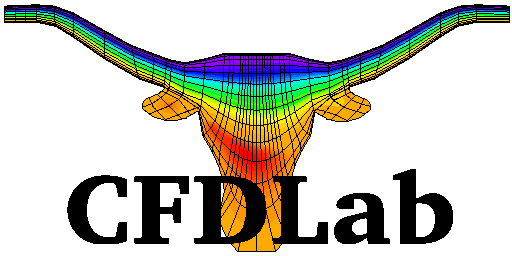
\includegraphics[width=.5in]{figures/cfdlab}}




%% Extra stuff we might find useful someday...

%% Example using multirow
%% \begin{frame}
%% \begin{tabular}{|l|l|l|}
%% \hline
%% \multicolumn{3}{|c|}{Team sheet} \\
%% \hline
%% %Goalkeeper & GK & Paul Robinson \\ \hline
%% \multirow{4}{*}{Defenders} & LB & Lucus Radebe \\
%%  & DC & Michael Duberry \\
%%  & DC & Dominic Matteo \\
%%  & RB & Didier Domi \\ \hline
%% \multirow{3}{*}{Midfielders} & MC & David Batty \\
%%  & MC & Eirik Bakke \\
%%  & MC & Jody Morris \\ \hline
%% Forward & FW & Jamie McMaster \\ \hline
%% \multirow{2}{*}{Strikers} & ST & Alan Smith \\
%%  & ST & Mark Viduka \\
%% \hline
%% \end{tabular}
%% \end{frame}










%% \begin{frame}%[t]
%%   %\frametitle{Surface-Tension-Driven Flow}
%%   \begin{center}
%%     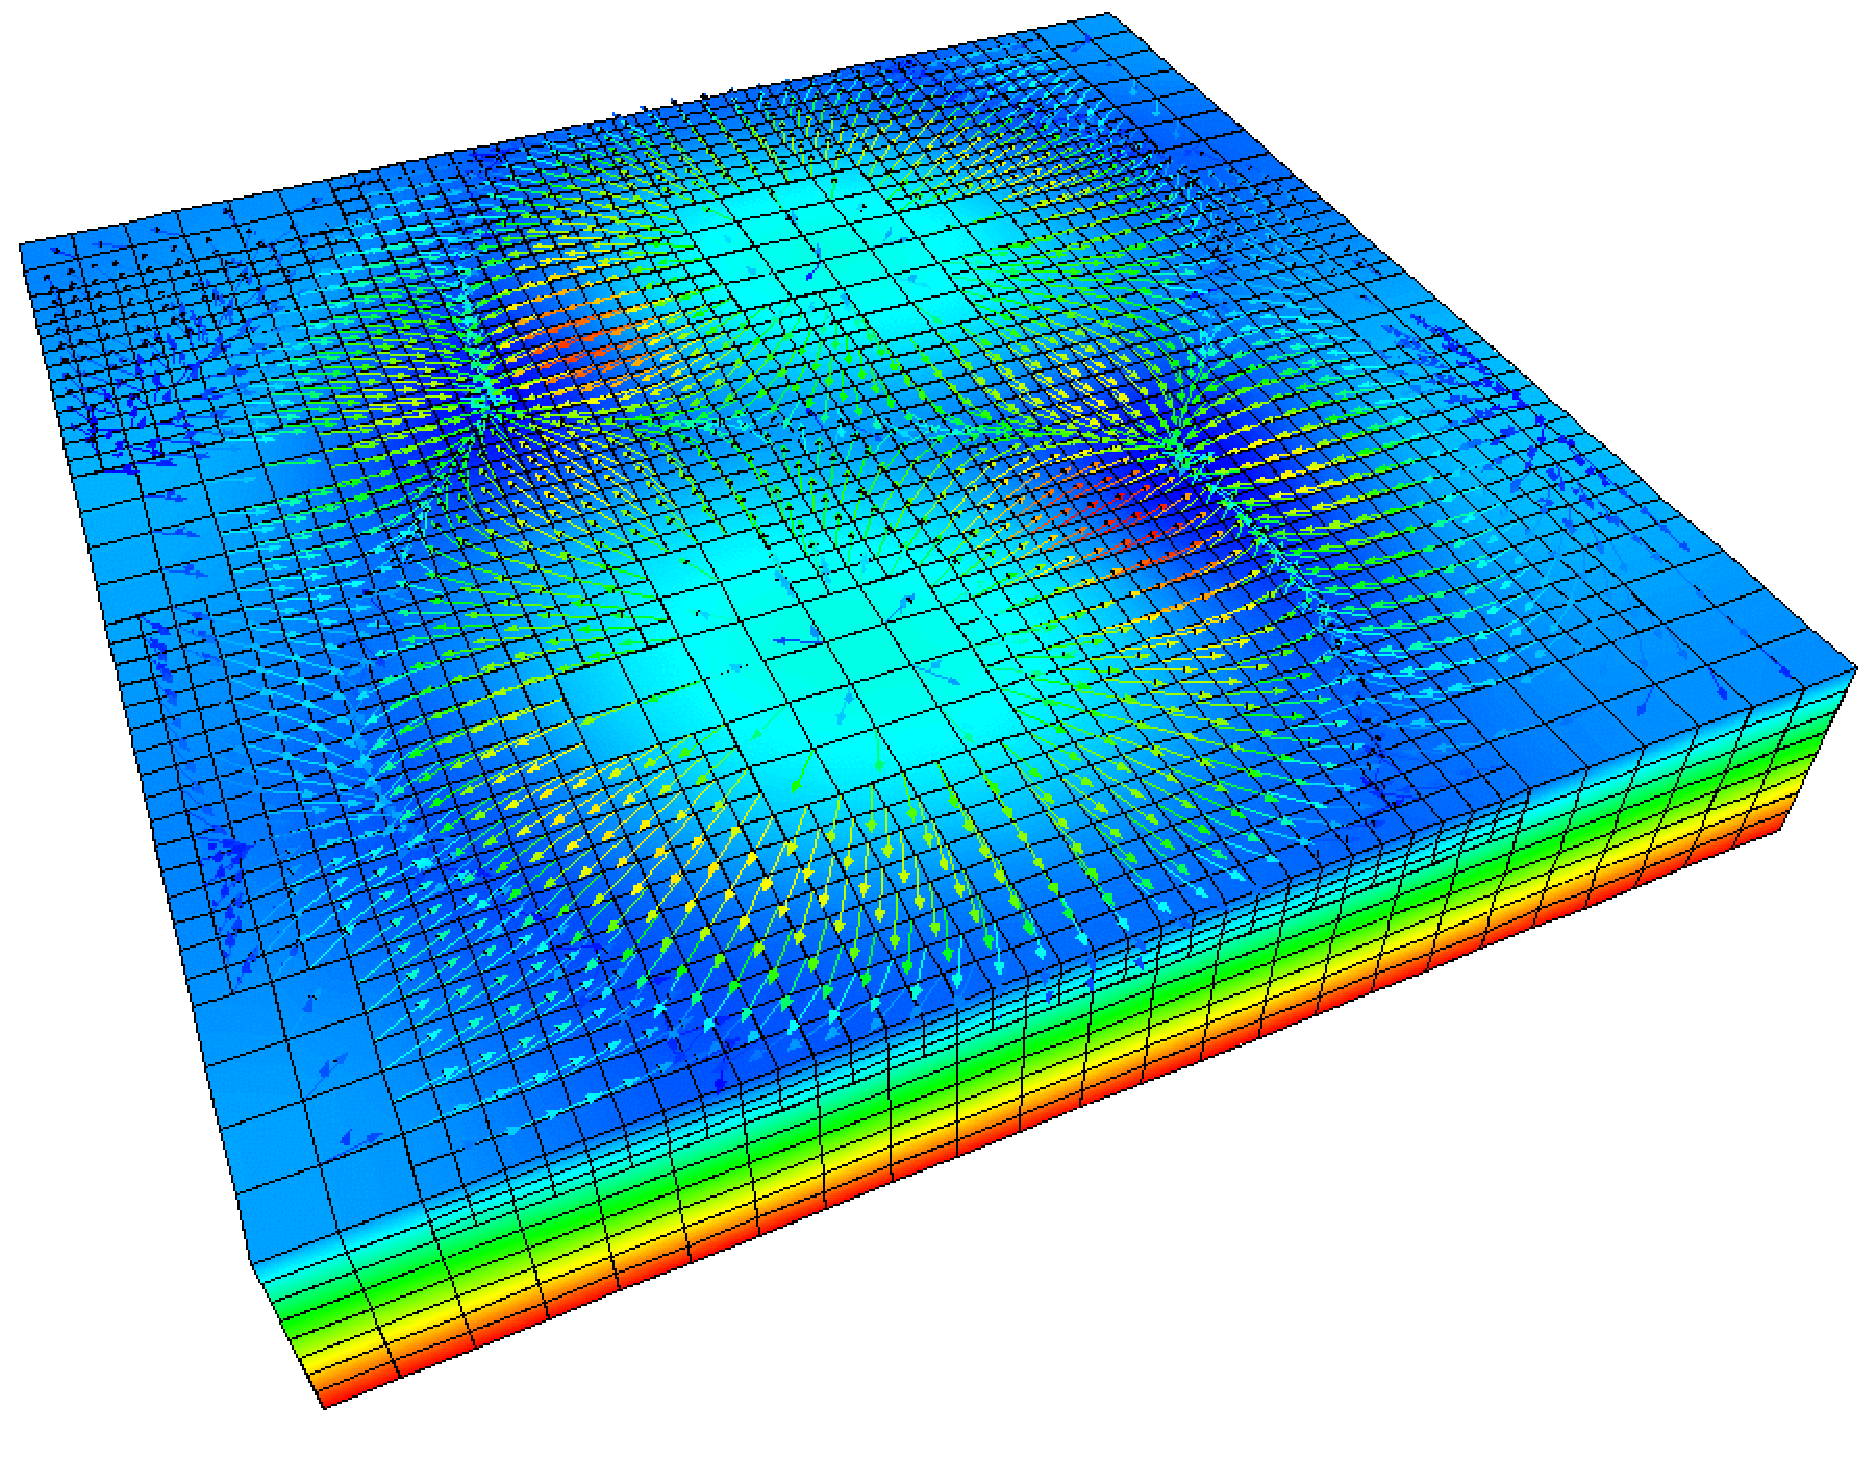
\includegraphics[width=.6\textwidth]{figures/rbm_adapt_soln}    
%%   \end{center}
%%   \vspace{-.25in}

%% %  \begin{block}{}
%%     \begin{itemize}
%%     \item{Adaptive grid solution shown
%%       with temperature contours and velocity vectors.      }
%%       \end{itemize}
%% %  \end{block}
%% \end{frame}








% Original movie inclusion code from Ben's defense
%\centerline{\includemovie[autoplay,loop,text={\includegraphics[height=.8\textheight]{figures/run2890_computed}}]{}{.8\textheight}{movies/Schlieren_run2890.avi}}



%% \begin{frame}
%%   % FIXME: place-holder image for when movie isn't playing?
%%   % setting height=.8\textwidth shrinks the whole movie
%%   % Does the ``poster'' option work?
%%   % Without an image in the text= argument, the movie is the size of the text ...
%%   % Without any text or image and no sizes given, the size is 0x0 ...
%%   % Options are \includemovie{width}{height}{filename}
%%   \centerline
%%       {
%%         \includemovie[autoplay,loop,text={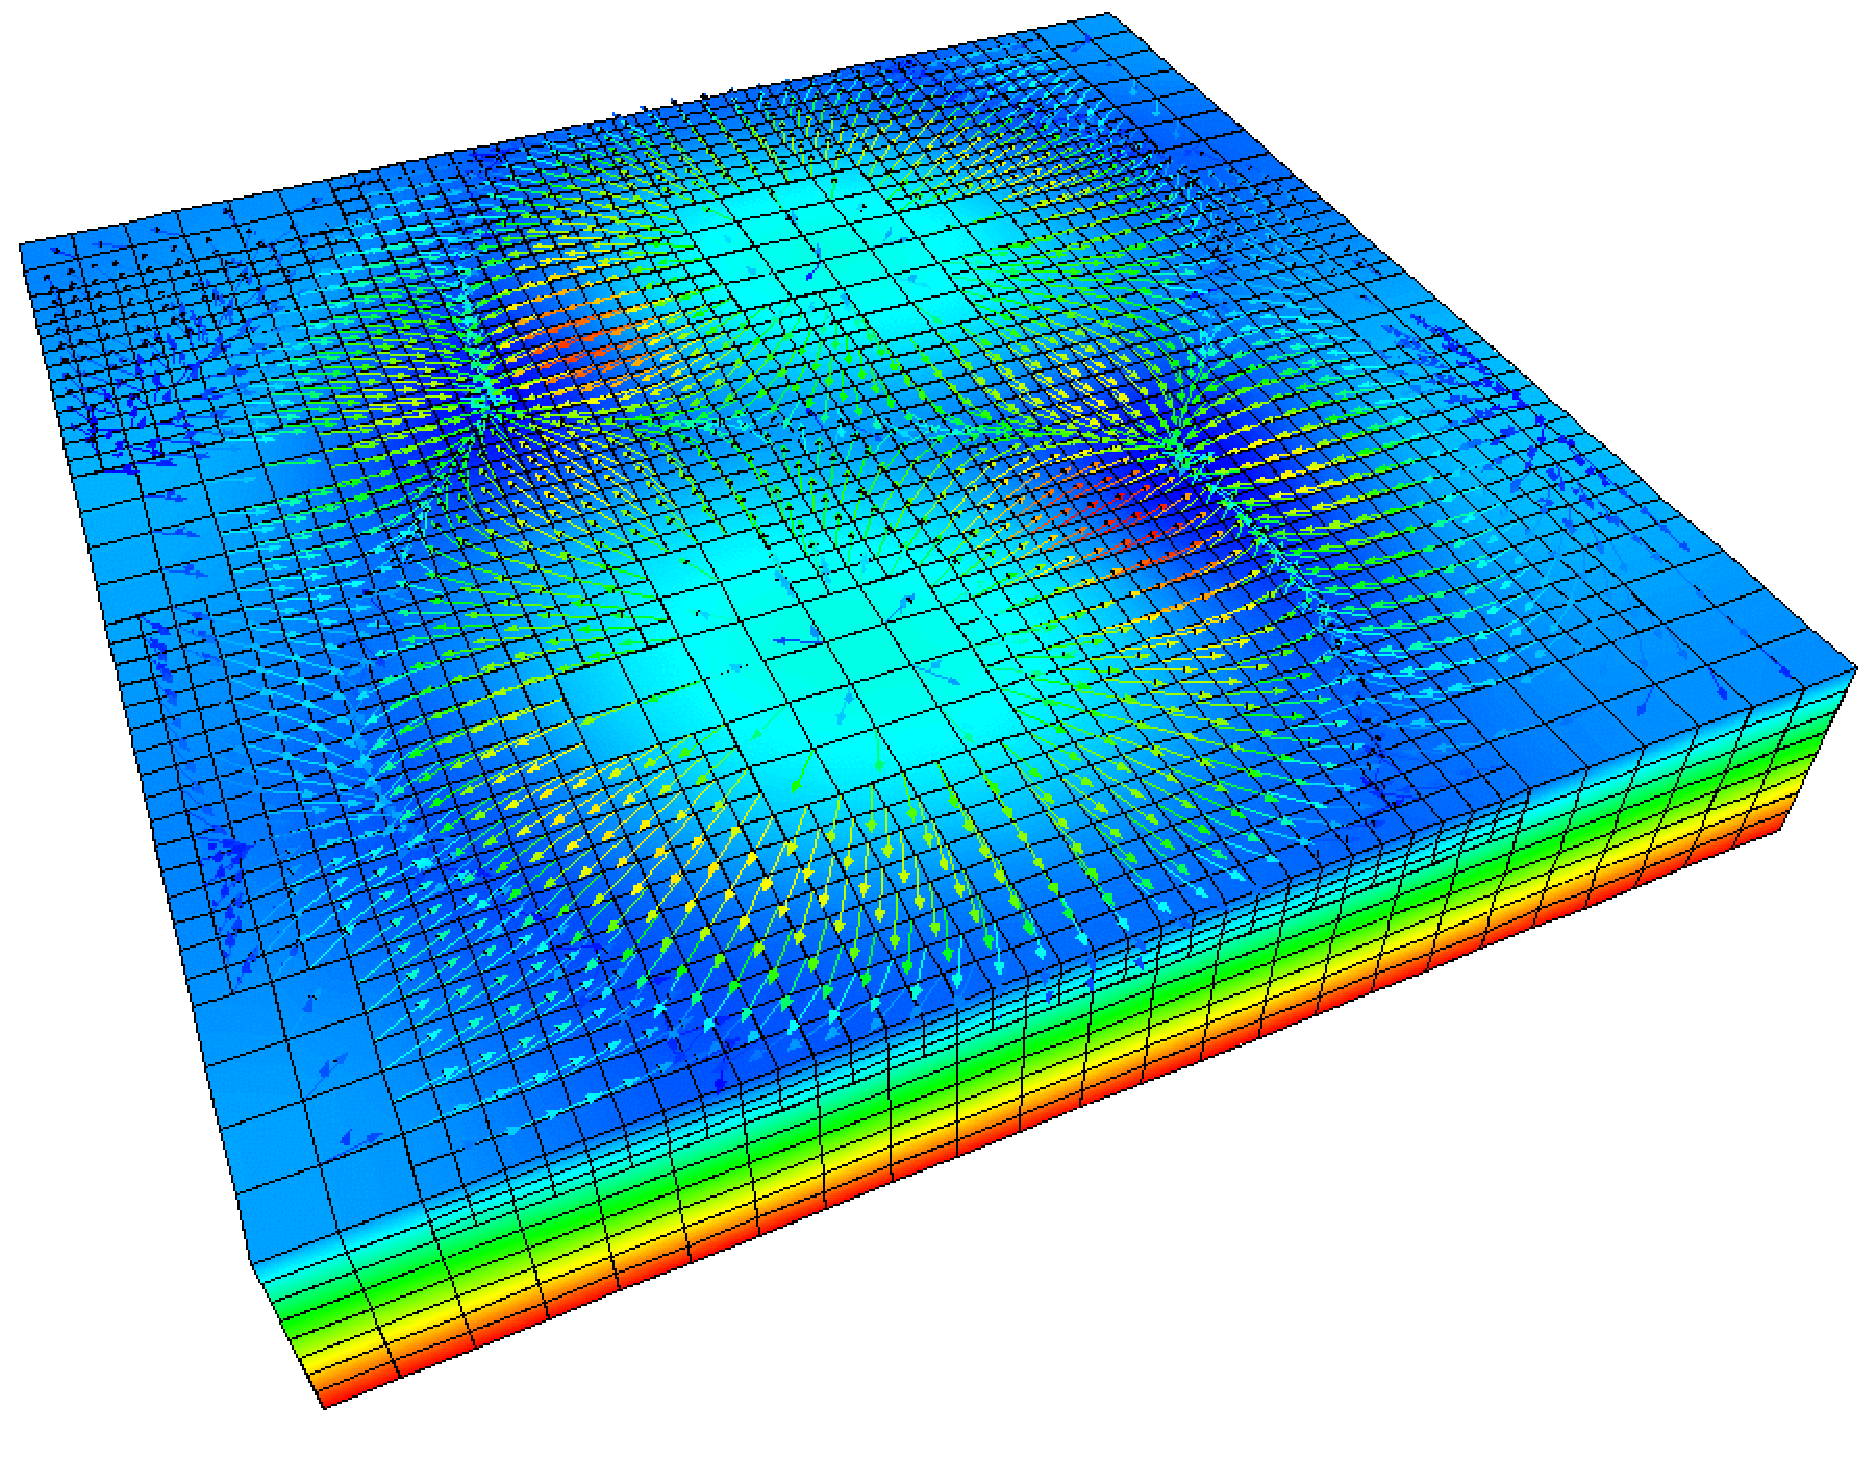
\includegraphics[width=.9\textwidth]{figures/rbm_adapt_soln}}]
%%                      {}{}{movies/Gamma_8_umovie_30x30.avi}
%%       }
%% \end{frame}



\begin{document}


 \begin{frame}
   \titlepage
 \end{frame}

\section*{Outline}% Make it easy to jump to this page in the PDF

% use outline_currentsection.tex to highlight the current section

% Auto-generate the TOC slide(s)
\begin{frame}
  %\tableofcontents[currentsection]
  \tableofcontents
\end{frame}

 

\section{Introduction}
\subsection*{What is LibMesh, and what does it do?}
\begin{frame}
  \begin{itemize}
  \itemsep=.75cm
  \item{An open-source (LGPL) finite element library.}
  \item{``Lowers the barrier of entry'' to serial and parallel
      simulation of multi-scale, multi-physics applications.}
  \item{Implements adaptive mesh refinement and coarsening on
      unstructured, hybrid grids in 1, 2, and 3D.}
  \item{\textbf{\texttt{libmesh.sf.net}}}
  \end{itemize}
\end{frame}

\subsection*{Natural Convection}
\begin{frame}[t]
  \begin{center}
    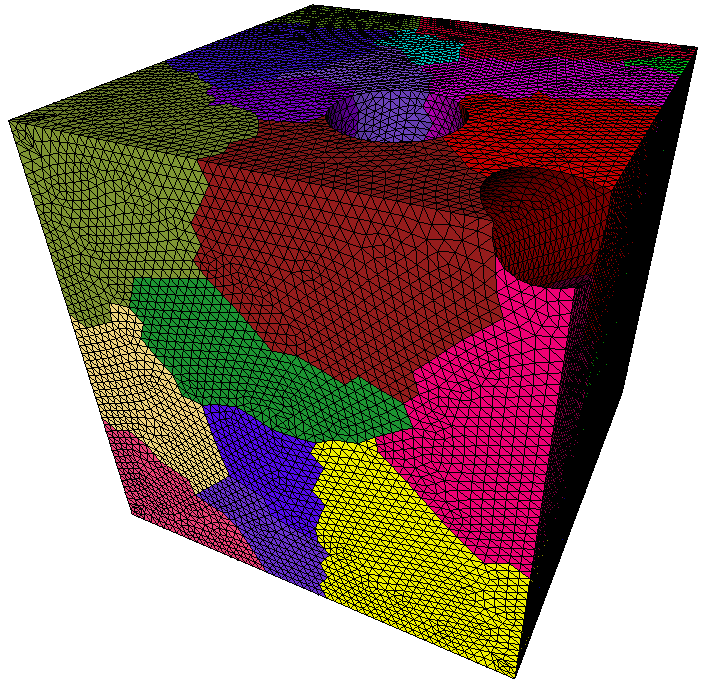
\includegraphics[width=.45\textwidth]{part_trans}
    %\\
    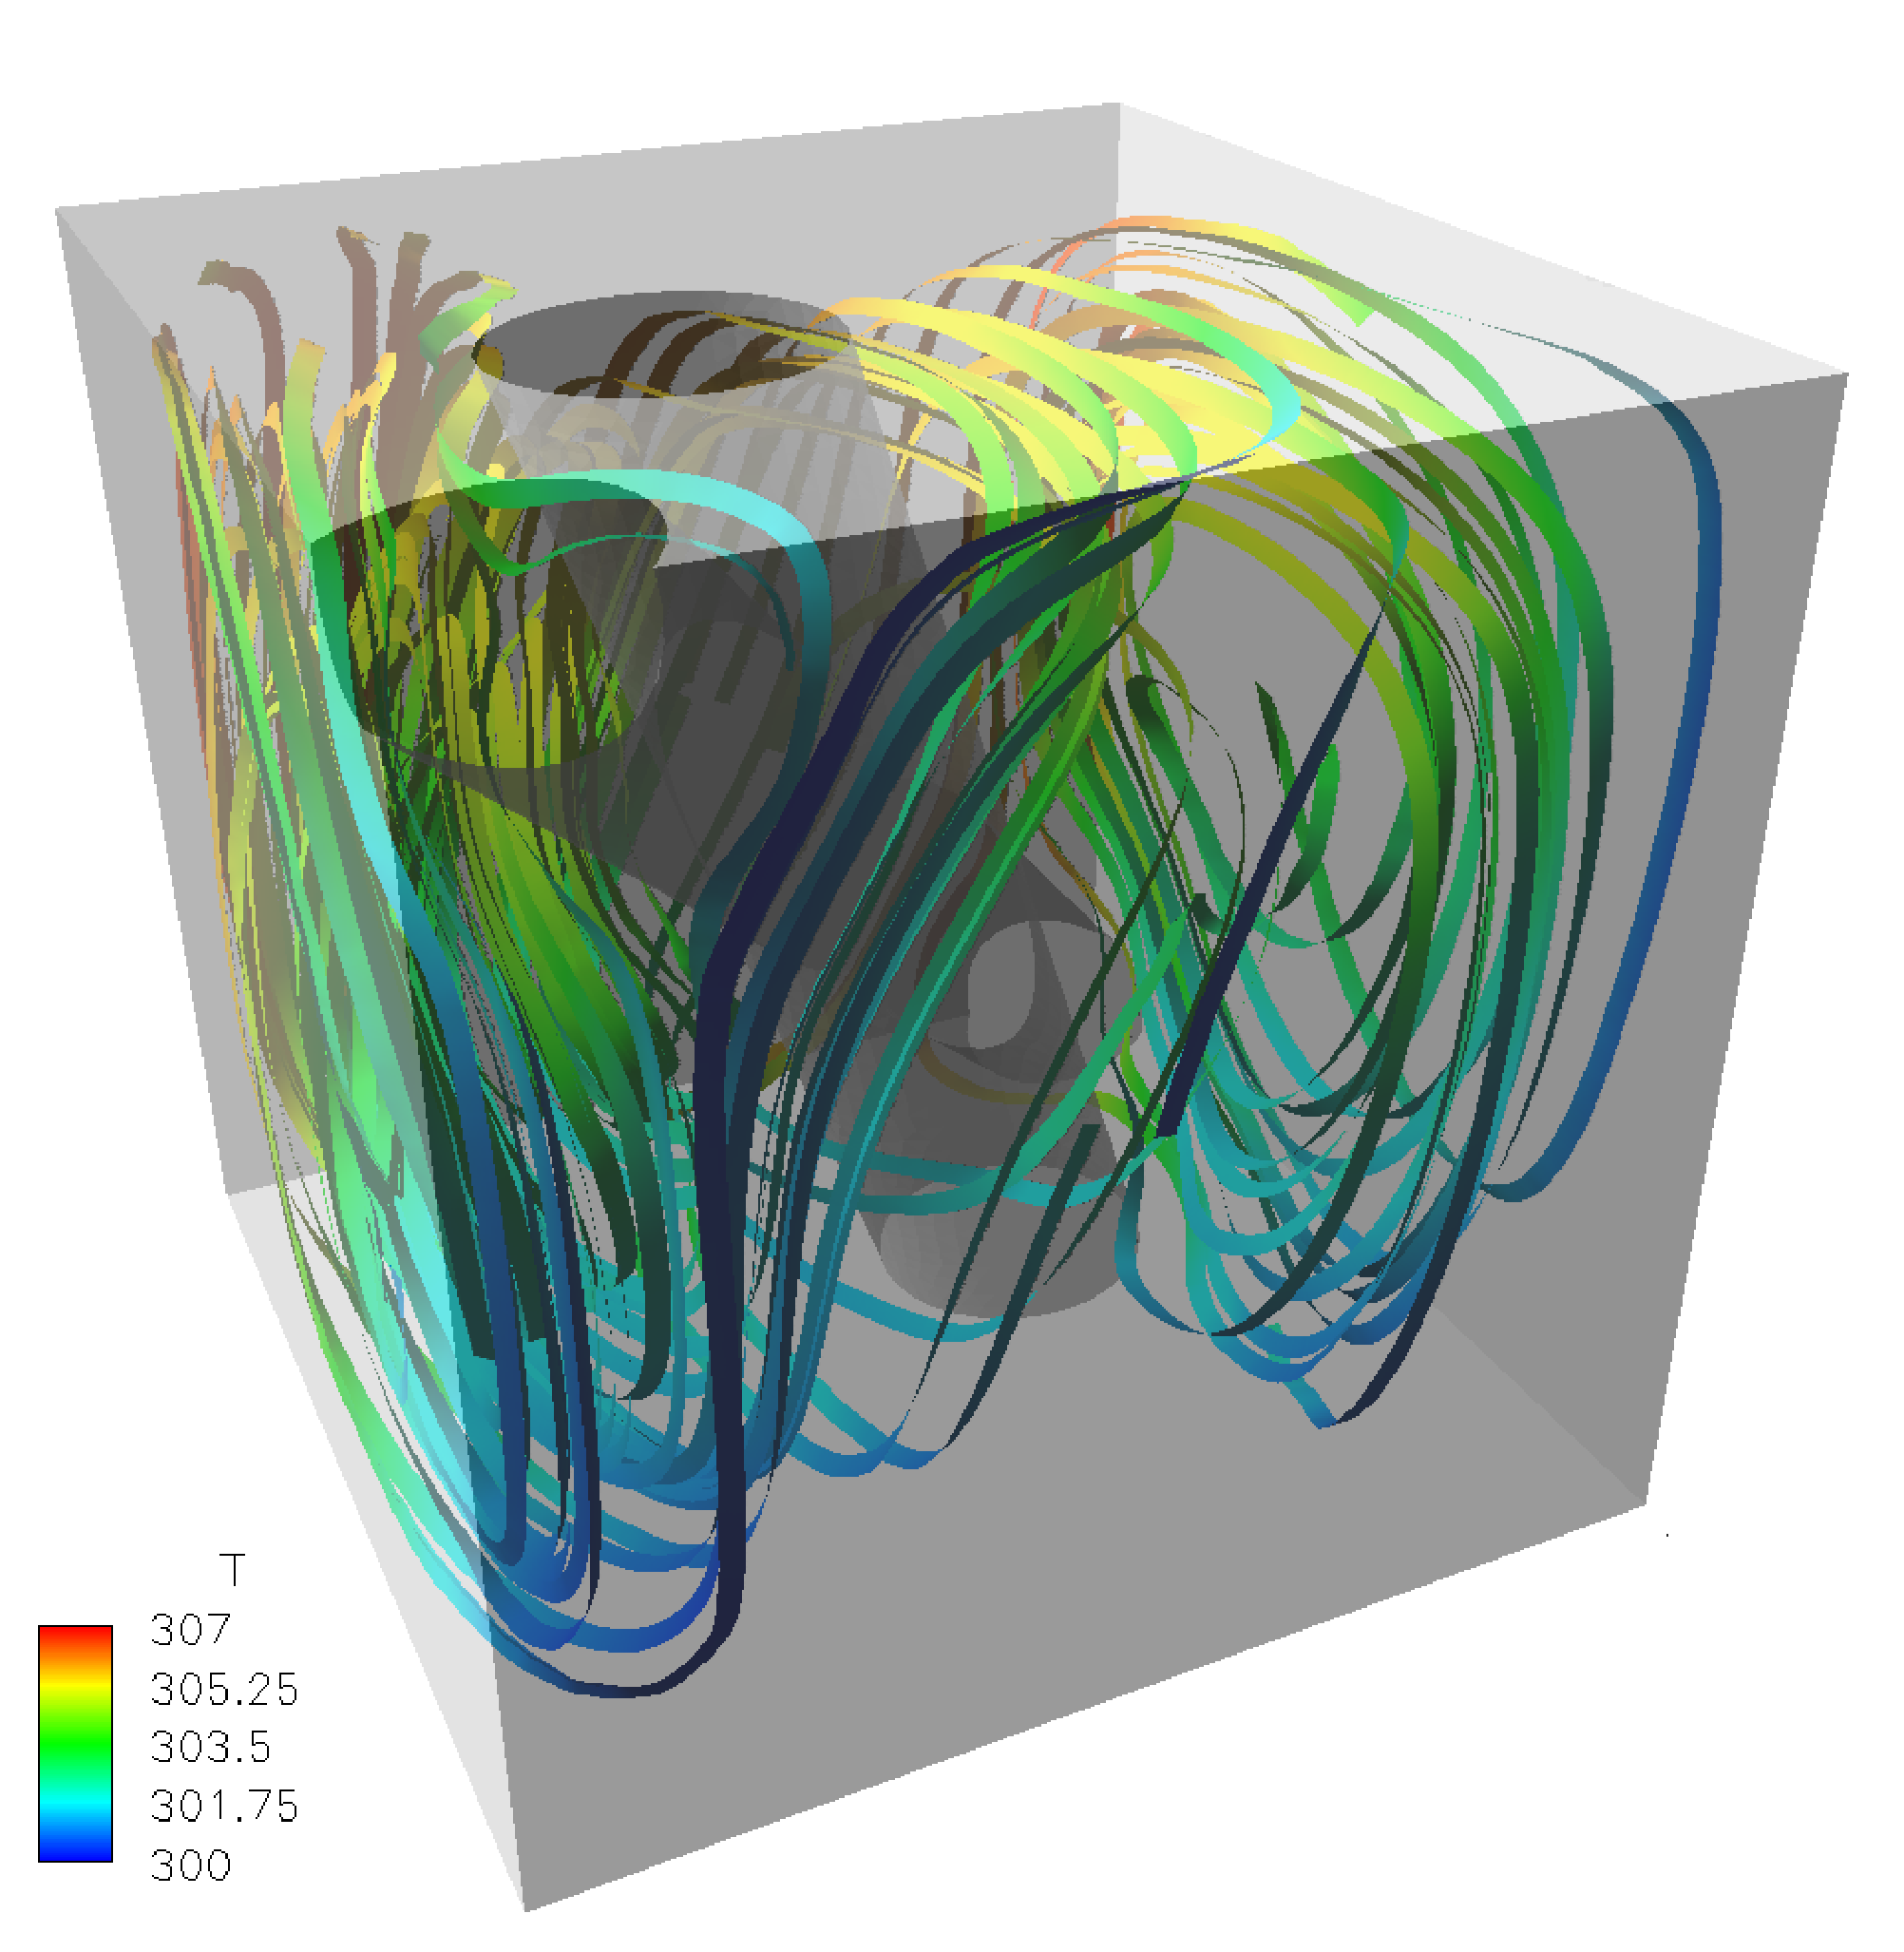
\includegraphics[width=.45\textwidth]{streamtraces}
  \end{center}
  \begin{block}{}
    \begin{itemize}
    \item{
      Tetrahedral mesh of ``pipe'' geometry.
      Stream ribbons colored by temperature.
      }
      \end{itemize}
  \end{block}
\end{frame}
 % Pretty picture

\subsection*{Who's responsible for this?}
\begin{frame}
  \begin{itemize}
    \itemsep=.5cm
  \item{Originated in the CFDLab, UT-Austin.}
    % \begin{itemize}
    % \item{University of Texas, Aerospace Engineering Department}
    % \end{itemize}
  \item{Started by \emph{B.~Kirk} (now at NASA) as part of PhD research.}
  \item{\emph{J.~Peterson} (TACC), first user, early class design/organization.}
  \item{Current lead developer is \emph{R.~Stogner} (ICES Post-doc, UT-Austin).}
  \item{Common PhD advisor: \emph{Graham F.\ Carey}}
  \end{itemize}
\end{frame}


\subsection*{Collaborators, past and present}
\begin{frame}
      \begin{itemize}
        \itemsep=.25cm
      \item {Daniel Dreyer and Steffen Petersen, TUHH
          %Technische Universit\"{a}t Hamburg-Harburg 
          % \url{http://www.tu-harburg.de}
          (Infinite Elements)
        }
        % 
      \item {Derek Gaston, INL
          (Mesh Redistribution)
        }
        %
      \item {David Knezevic, MIT (1D support, Adaptive Mesh I/O) }
        %
      \item {Tim Kr\"{o}ger, Universit\"{a}t Bremen 
          % \url{http://www.uni-bremen.de/}
          % tim.kroeger@cevis.uni-bremen.de
          (Shell Matrices, Ghosted Vectors)
        }
        %
      \item{Many others: A.~Coutinho, O.~Certik, M.~L\"{u}thi, W.~Ruijter, J.~Roman, V.~Mahadevan, V.~Garg, V.~Carey, \ldots }
      \end{itemize}
\end{frame}

\subsection*{Scope of the library}
\begin{frame}%[<+->]
  %\begin{block}{\texttt{libMesh} is not}
LibMesh is not
  \begin{itemize}
  \item {A physics implementation.}
  \item {A stand-alone application.}
  \end{itemize}
%  \end{block}
\vspace{1cm}
%  \begin{block}{\texttt{libMesh} is}
LibMesh is  \begin{itemize}
  \item {A software library and toolkit.}
  \item {Classes and functions for writing parallel adaptive finite element applications.}
  \item {An interface to linear algebra, meshing, partitioning, etc. libraries.}
  \end{itemize}
%  \end{block}
\end{frame}

\subsection*{Library Description}
\begin{frame}[t]
  %\frametitle{LibMesh Tree}
%  \vspace{-.25in}
%  \begin{center}
%    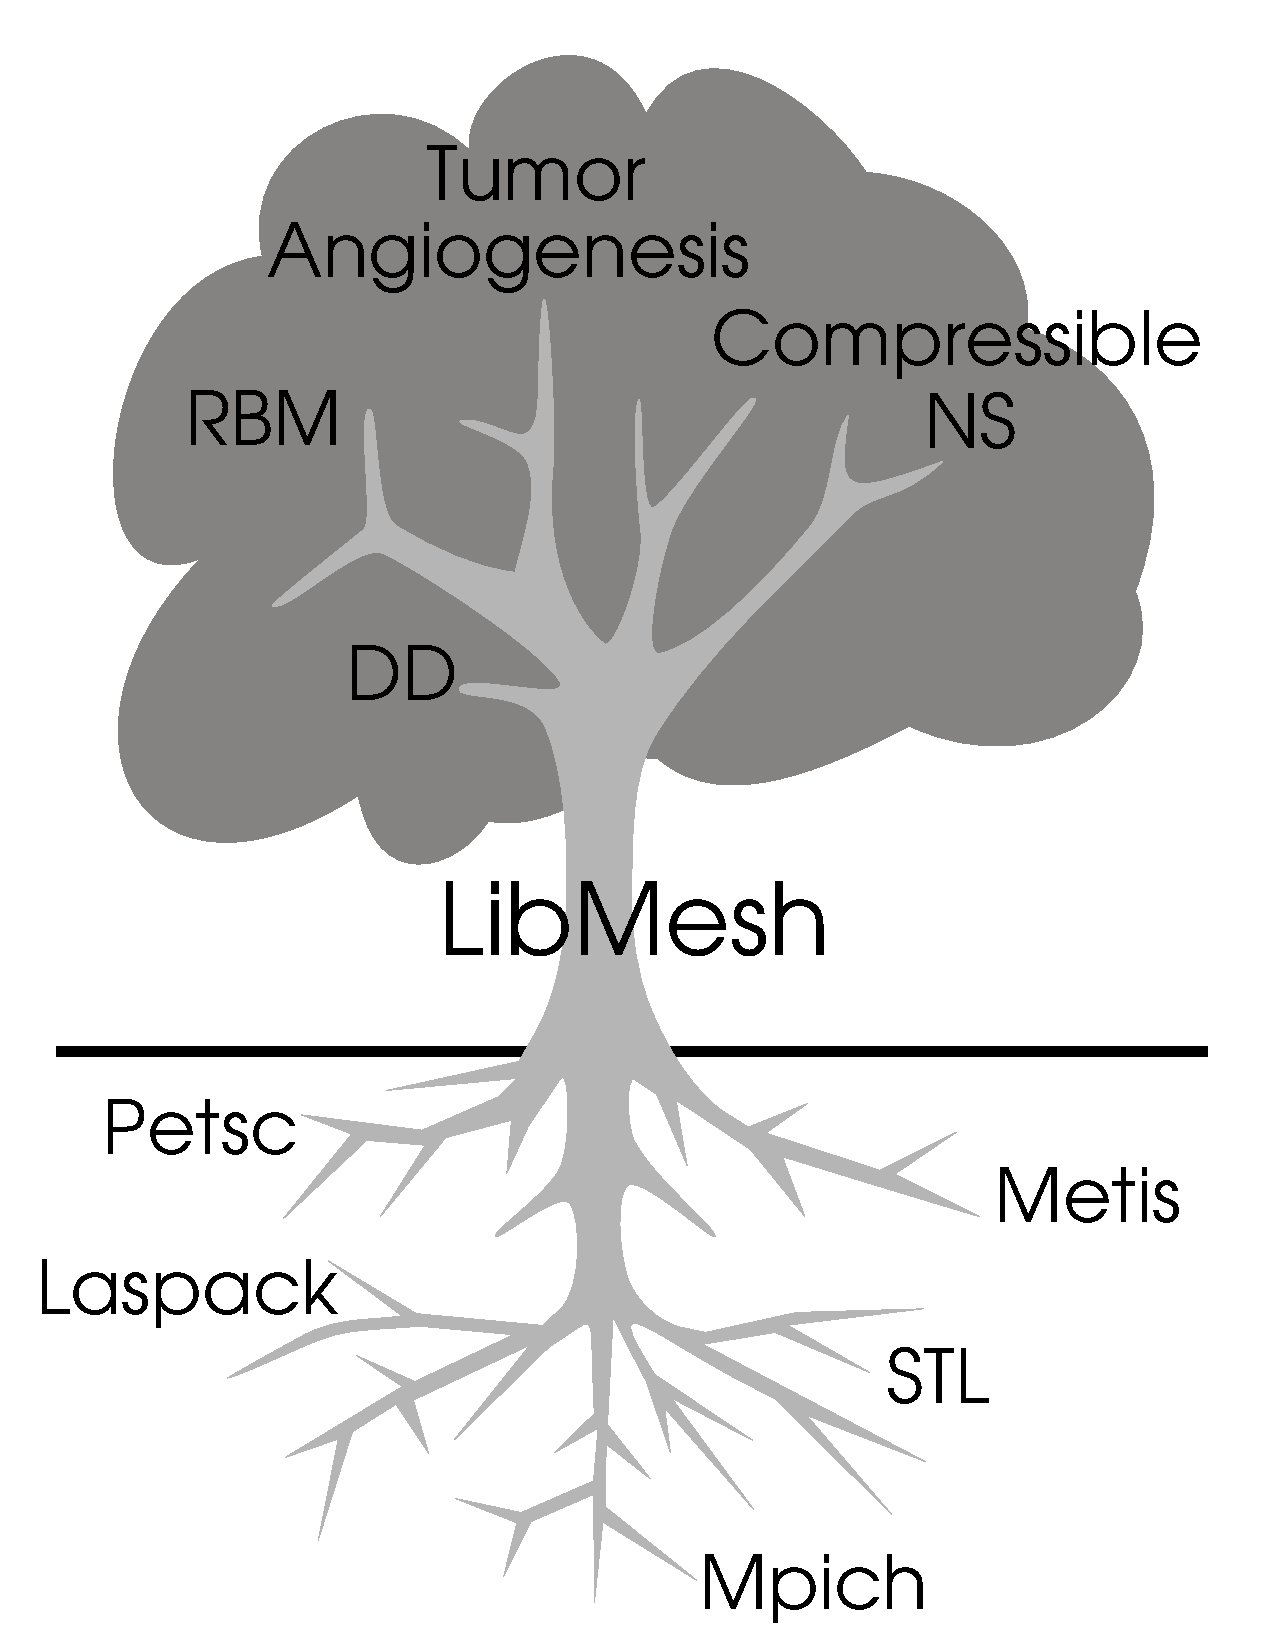
\includegraphics[width=.6\textwidth]{figures/mytreeandroots_allnames}    
%  \end{center}


    \begin{minipage}[h]{.6\textwidth}
    \begin{center}
      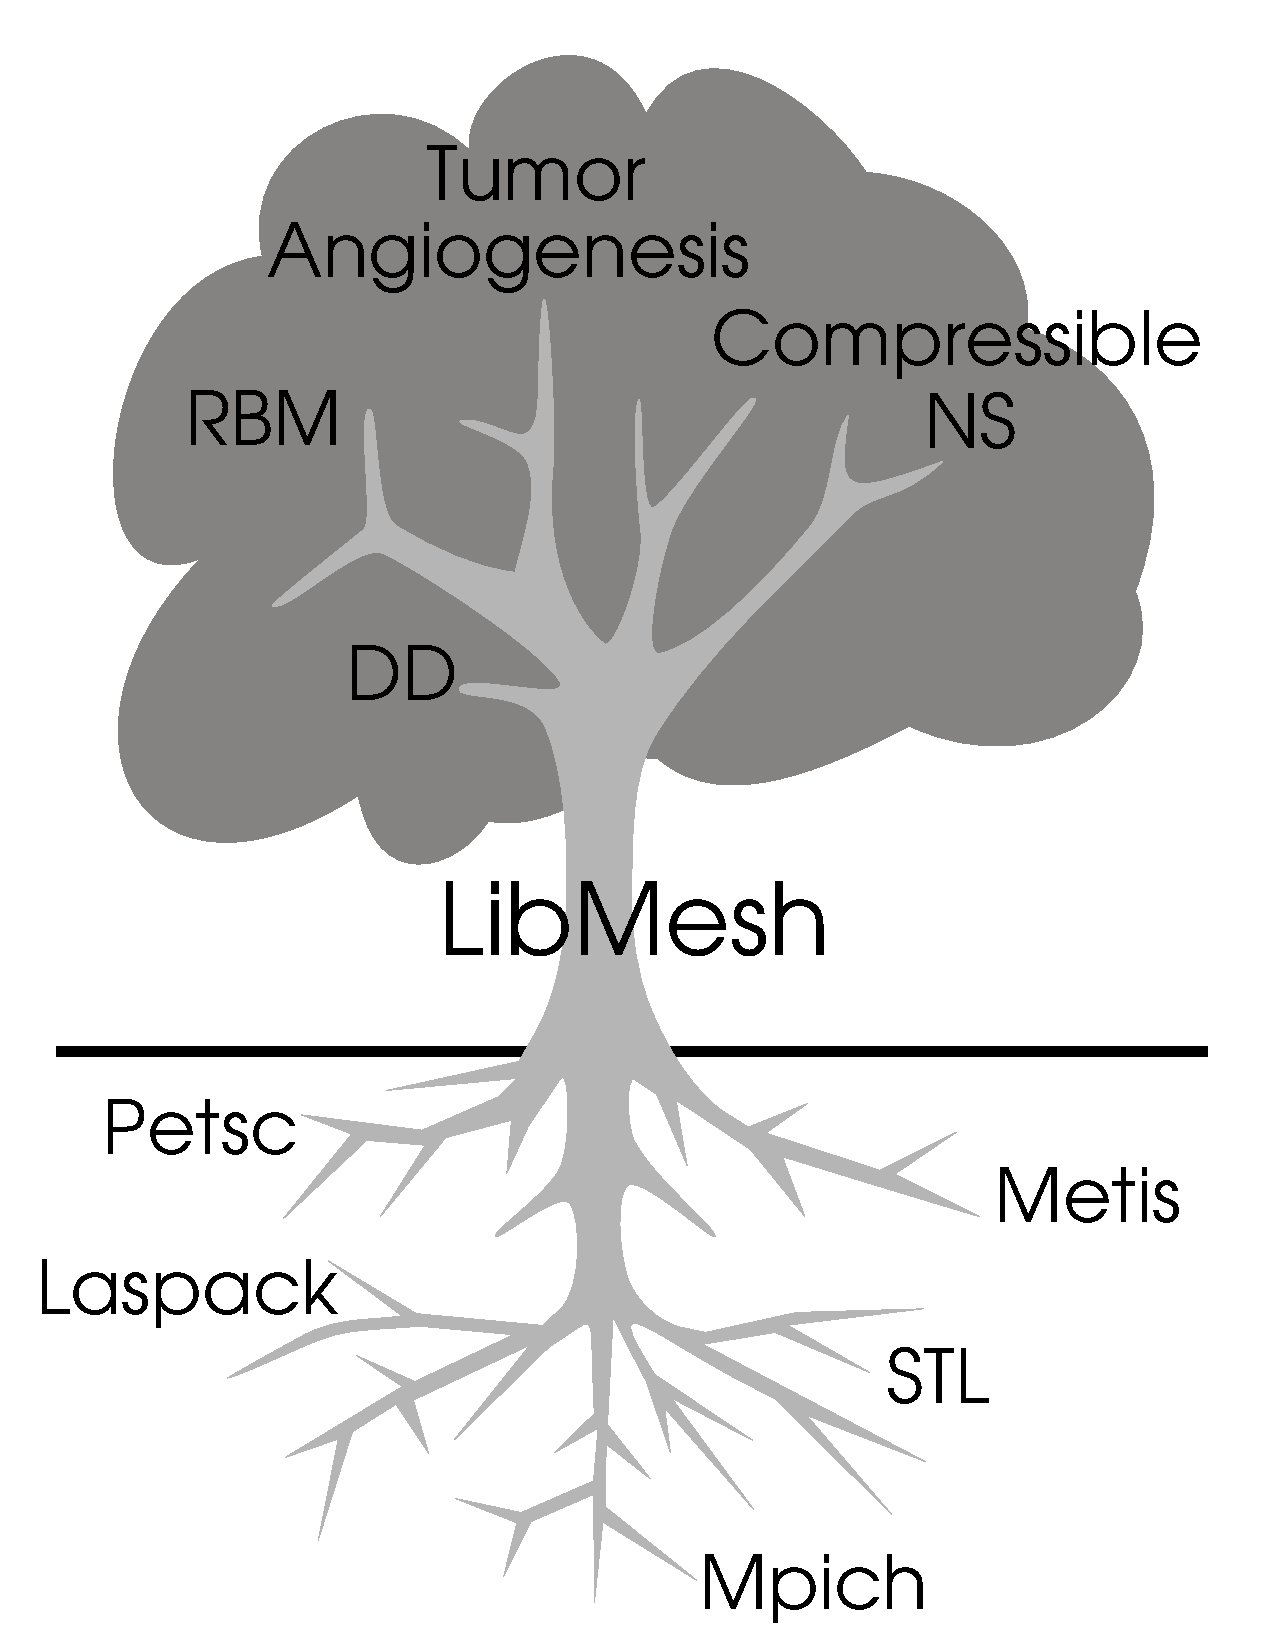
\includegraphics[width=.9\textwidth]{figures/mytreeandroots_allnames}
    \end{center}
  \end{minipage}
  \begin{minipage}[h]{.35\textwidth}
    \begin{block}{Library Structure}
      \begin{itemize}
        %\small
    \item Basic libraries are \LibMesh's ``roots''
    \item Application ``branches'' built off the library ``trunk''
      \end{itemize}
    \end{block}
  \end{minipage}



\end{frame}

\subsection*{What class of problems is LibMesh designed to solve?}
% The ``Generic BVP'' slide has been slightly revamped for notational consistency
\begin{frame}[t]
  %\frametitle{A Generic BVP}
  \begin{columns}[t]
    \column{.5\textwidth}
     \begin{itemize}
      \item General boundary value problems of the form:
      \end{itemize}
%    \begin{block}{}%{We assume there is a Boundary Value Problem of the form}
      \vspace{-.1in}
        \begin{eqnarray}
	\label{eqn:general_pde}
	\nonumber
	M \frac{\partial u}{\partial t} & = & F( u ) \;\;\;\; \in \Omega
        \\
	\nonumber
	G( u ) & = & 0 \;\;\;\;\;\;\;\;\; \in \Omega
	\\
	\nonumber
	u & = & u_D \;\;\;\;\;\;\; \in \partial \Omega_D
	\\
	\nonumber
	N(u) & = & 0 \;\;\;\;\;\;\;\;\; \in \partial \Omega_N
 	\\
 	\nonumber
 	u(\bv{x}, 0) & = & u_0(\bv{x}) 
      \end{eqnarray}
%    \end{block}
    %\pause
    \column{.5\textwidth}
      \begin{center}
	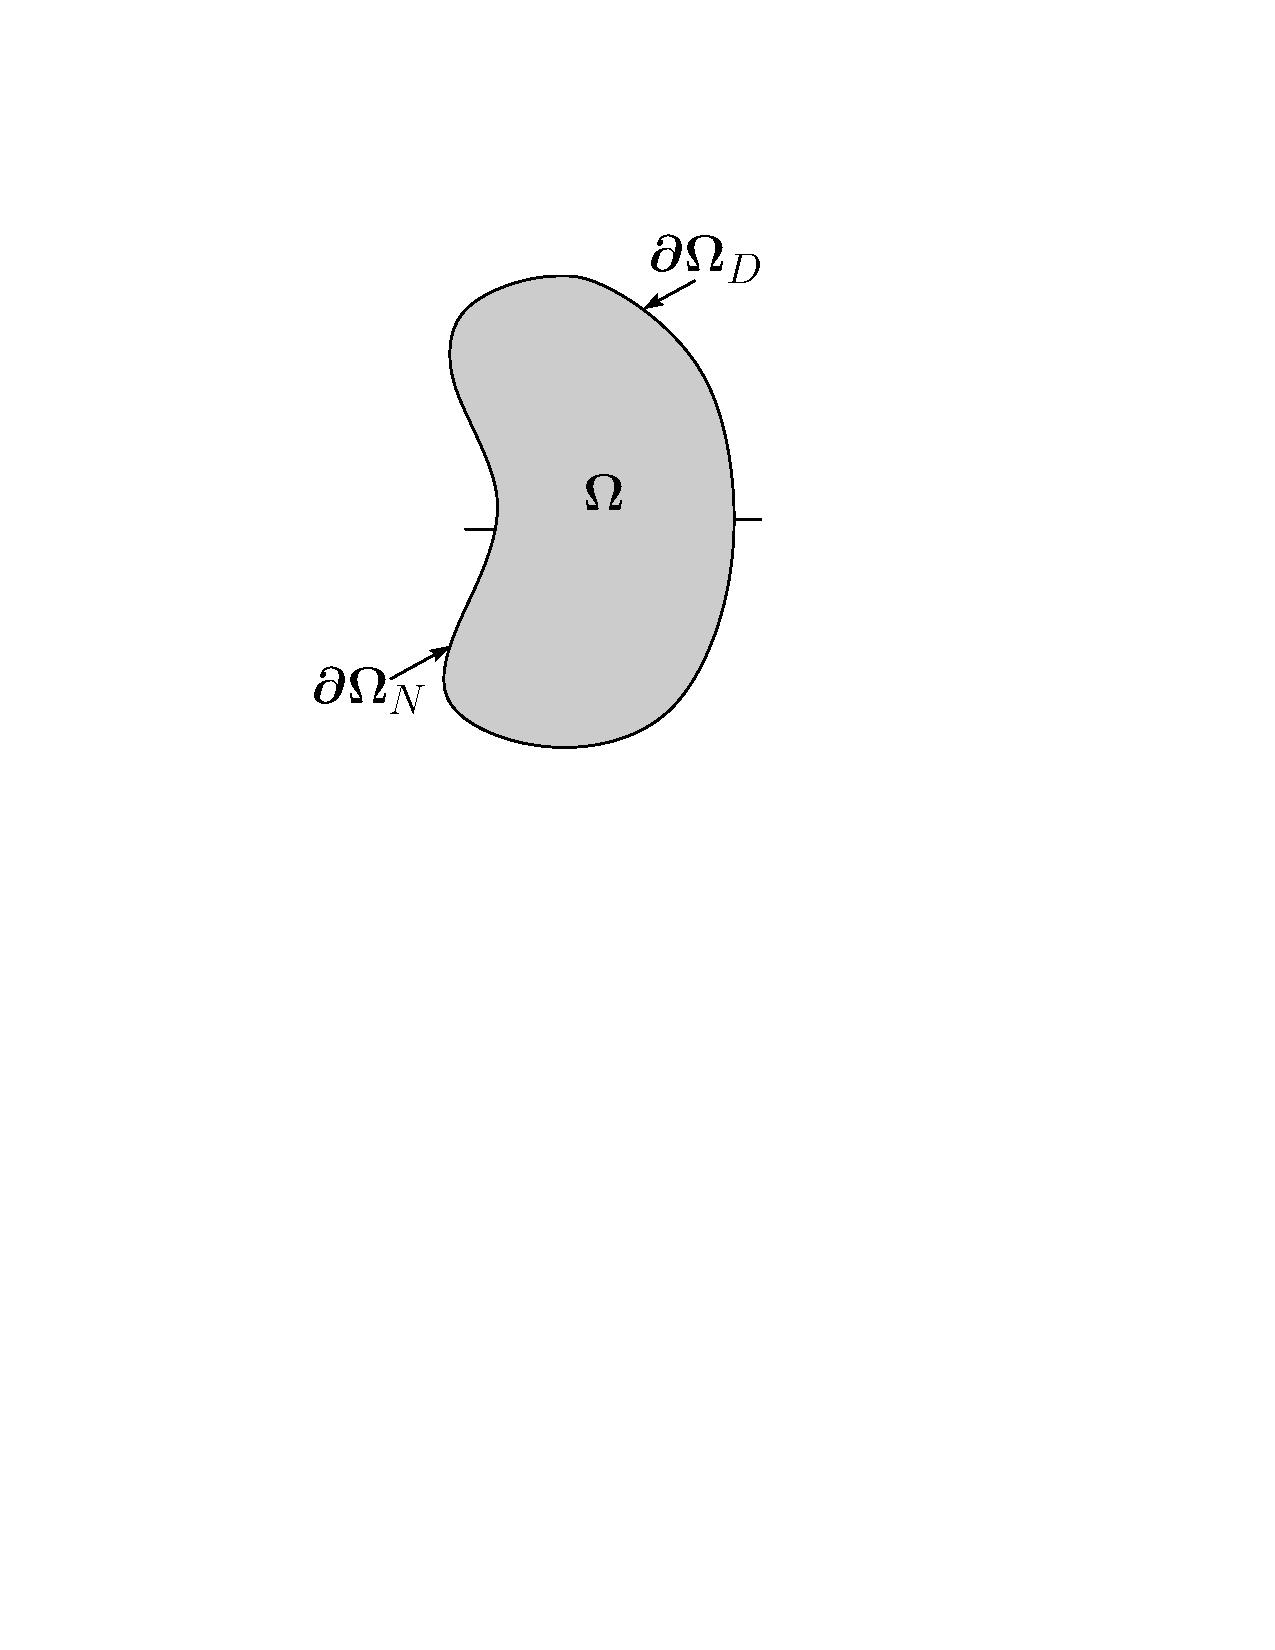
\includegraphics[viewport=140 420 400 685,clip=true,width=2in]{figures/domain2/domain2_input}
      \end{center}
  \end{columns}
\end{frame}

\begin{frame}
  %\frametitle{}
  \begin{columns}[t]
    \column{.5\textwidth}
    \begin{block}{}%A general class of PDE}
      \begin{itemize}
      \item{
	Associated to the problem domain $\Omega$ is a LibMesh data
	structure called a \texttt{Mesh}
      }
	
      \item{A \texttt{Mesh} is essentially
	a collection of finite elements}
      \end{itemize}
      \begin{equation}
	\label{eqn:discretized_domain}
	\nonumber
	\Omega^h:=\bigcup_e \Omega_e
      \end{equation}
    \end{block}
    %\pause
    \column{.5\textwidth}
    %\begin{block}{}
      \begin{center}
	%\fbox{
	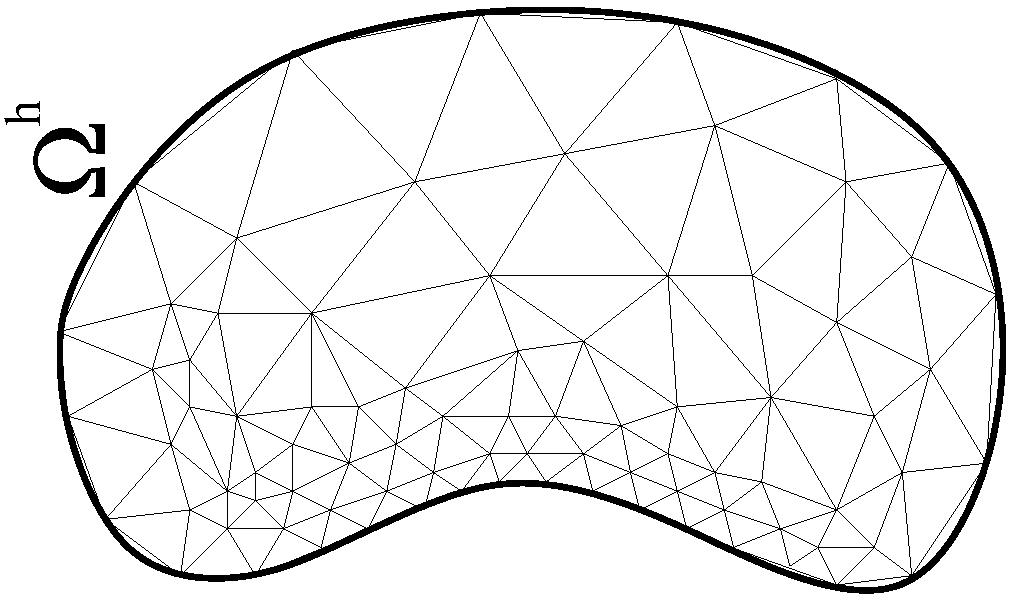
\includegraphics[width=2in,angle=-90]{discretized_domain}
	%}
      \end{center}
    %\end{block}
  \end{columns}
  \visible<2>
  {
  \begin{itemize}
    \item{LibMesh provides some simple structured mesh generation
routines, file inputs, and interfaces to Triangle and TetGen.}
  \end{itemize}
  }
\end{frame}


\begin{frame}[shrink]
  \frametitle{The Mesh}
  
  \lstinputlisting[language=C++]{snippets/mesh.cxx}

\end{frame}

\begin{frame}
\begin{minipage}[h]{.65\textwidth}
\begin{center}
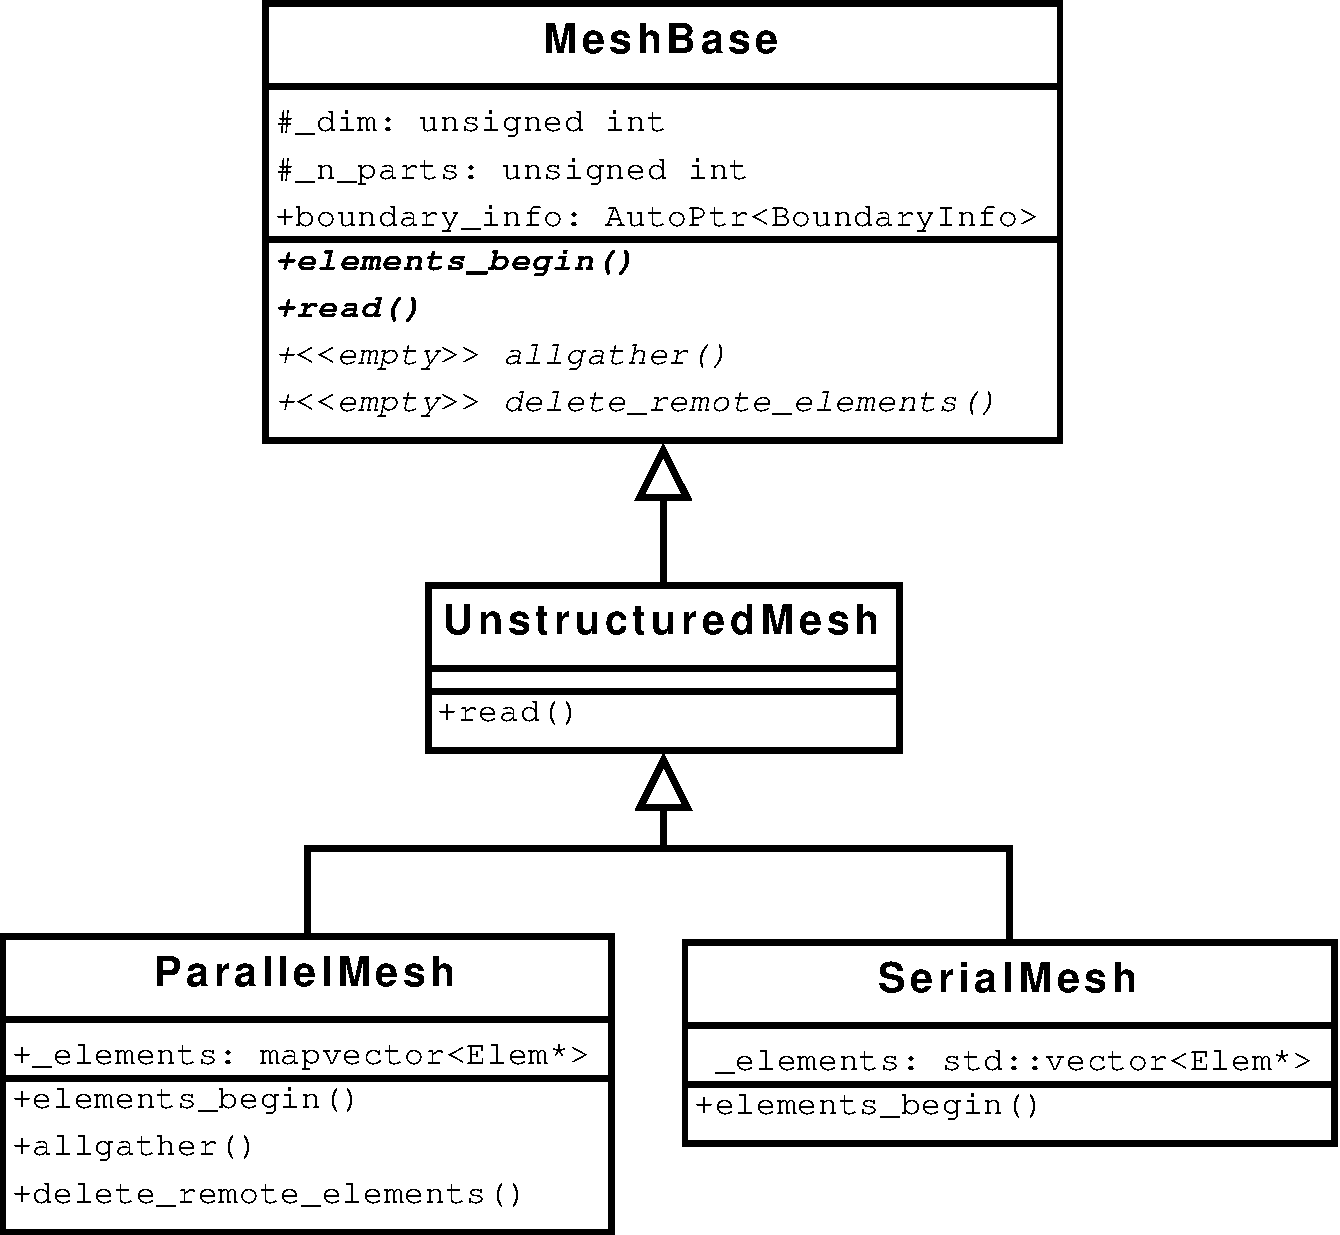
\includegraphics[width=.95\textwidth]{figures/Mesh}
\end{center}
\end{minipage}
\begin{minipage}[h]{.3\textwidth}
%\begin{block}{}
\begin{itemize}
\item Serial \texttt{Mesh} recently extended to Parallel
\item Serial functionality still present \& interchangeable
\end{itemize}
%\end{block}
\end{minipage}

\end{frame}

\subsection*{BVP framework: The FEMSystem class}

\begin{frame}
  \begin{minipage}[h]{.45\textwidth}
    \begin{center}
      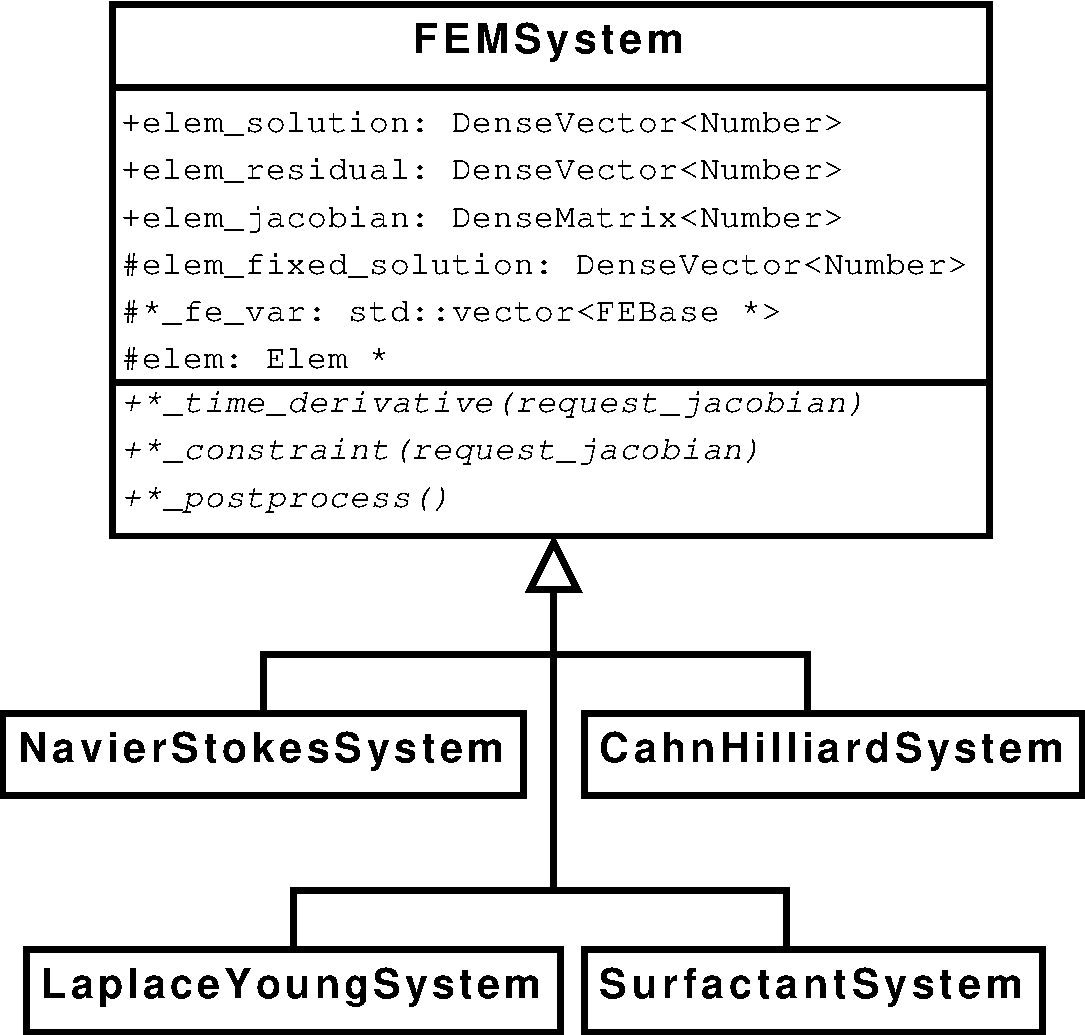
\includegraphics[width=.9\textwidth]{figures/FEMSystem}
    \end{center}
  \end{minipage}
  \begin{minipage}[h]{.5\textwidth}
      \begin{itemize}
      %\item Generalized IBVP representation
      %\item FEMSystem does all initialization, global assembly
      \item
        User provides (weak form) weighted residuals
        \begin{equation}
          \nonumber
        \left(M\frac{\partial u}{\partial t}, v_i \right) =
        \left(F\left(u\right), v_i\right)
          \end{equation}
        \item And/or constraints
        \begin{equation}
          \nonumber
          \left(G\left(u\right), v_i\right) = 0
        \end{equation}
      \end{itemize}
  \end{minipage}
\end{frame}

\subsection*{Weighted Residual Statement}
\begin{frame}%[<+->]
  %\frametitle{Poisson Equation}
  \begin{itemize}
  \item {For simplicity we start with the weighted
    residual statement arising from the Poisson equation,
    with $\partial \Omega_N = \emptyset$, 
    \begin{eqnarray}
      \nonumber
      (F( u^h ), v^h) := \hspace{2.5in} \\  \nonumber
      \int_{\Omega^h}  \left[ \nabla u^h \cdot \nabla v^h - fv^h \right] dx %\\ \nonumber
      %+ \int_{\partial \Omega^h_N} u_N v^h \;ds
      =0 \hspace{.5in} \forall v^{h} \in \mathcal{V}^{h}
    \end{eqnarray}
  }
  \end{itemize}
\end{frame}

\begin{frame}[fragile,t]  
%  \frametitle{Poisson Equation}
%	\begin{block}{}
	  \begin{itemize}    
	  \item{ The LibMesh representation of the matrix and
	    rhs assembly is similar to the mathematical statements.
	  }
	  \end{itemize}
%	\end{block}
\small
\begin{semiverbatim}
for (q=0; q<Nq; ++q) 
  for (i=0; i<Ns; ++i) \{
    \alert<2>{Fe(i)   += JxW[q]*f(xyz[q])*phi[i][q];}
    
    for (j=0; j<Ns; ++j)
      \alert<3>{Ke(i,j) += JxW[q]*(dphi[j][q]*dphi[i][q]);}
  \}
\end{semiverbatim}
\only<2>
{
  \begin{equation}
    \nonumber
    \bv{F}^e_{i} = 
    \sum_{q=1}^{N_q}
    f(x(\xi_q))
    \phi_i(\xi_q)
    |J(\xi_q)| w_q
  \end{equation}
}
\only<3->
{
  \begin{equation}
  \nonumber
  \bv{K}^e_{ij} =
  \sum_{q=1}^{N_q}
    \nabla \phi_j(\xi_q) \cdot
    \nabla \phi_i(\xi_q)
    |J(\xi_q)| w_q
  \end{equation}
}
\end{frame}

\subsection*{Compressible Navier-Stokes}
\begin{frame}
    \begin{figure}[!htb]
      \begin{center}
        \subfigure{\label{fig:fob_uniform_2_sol}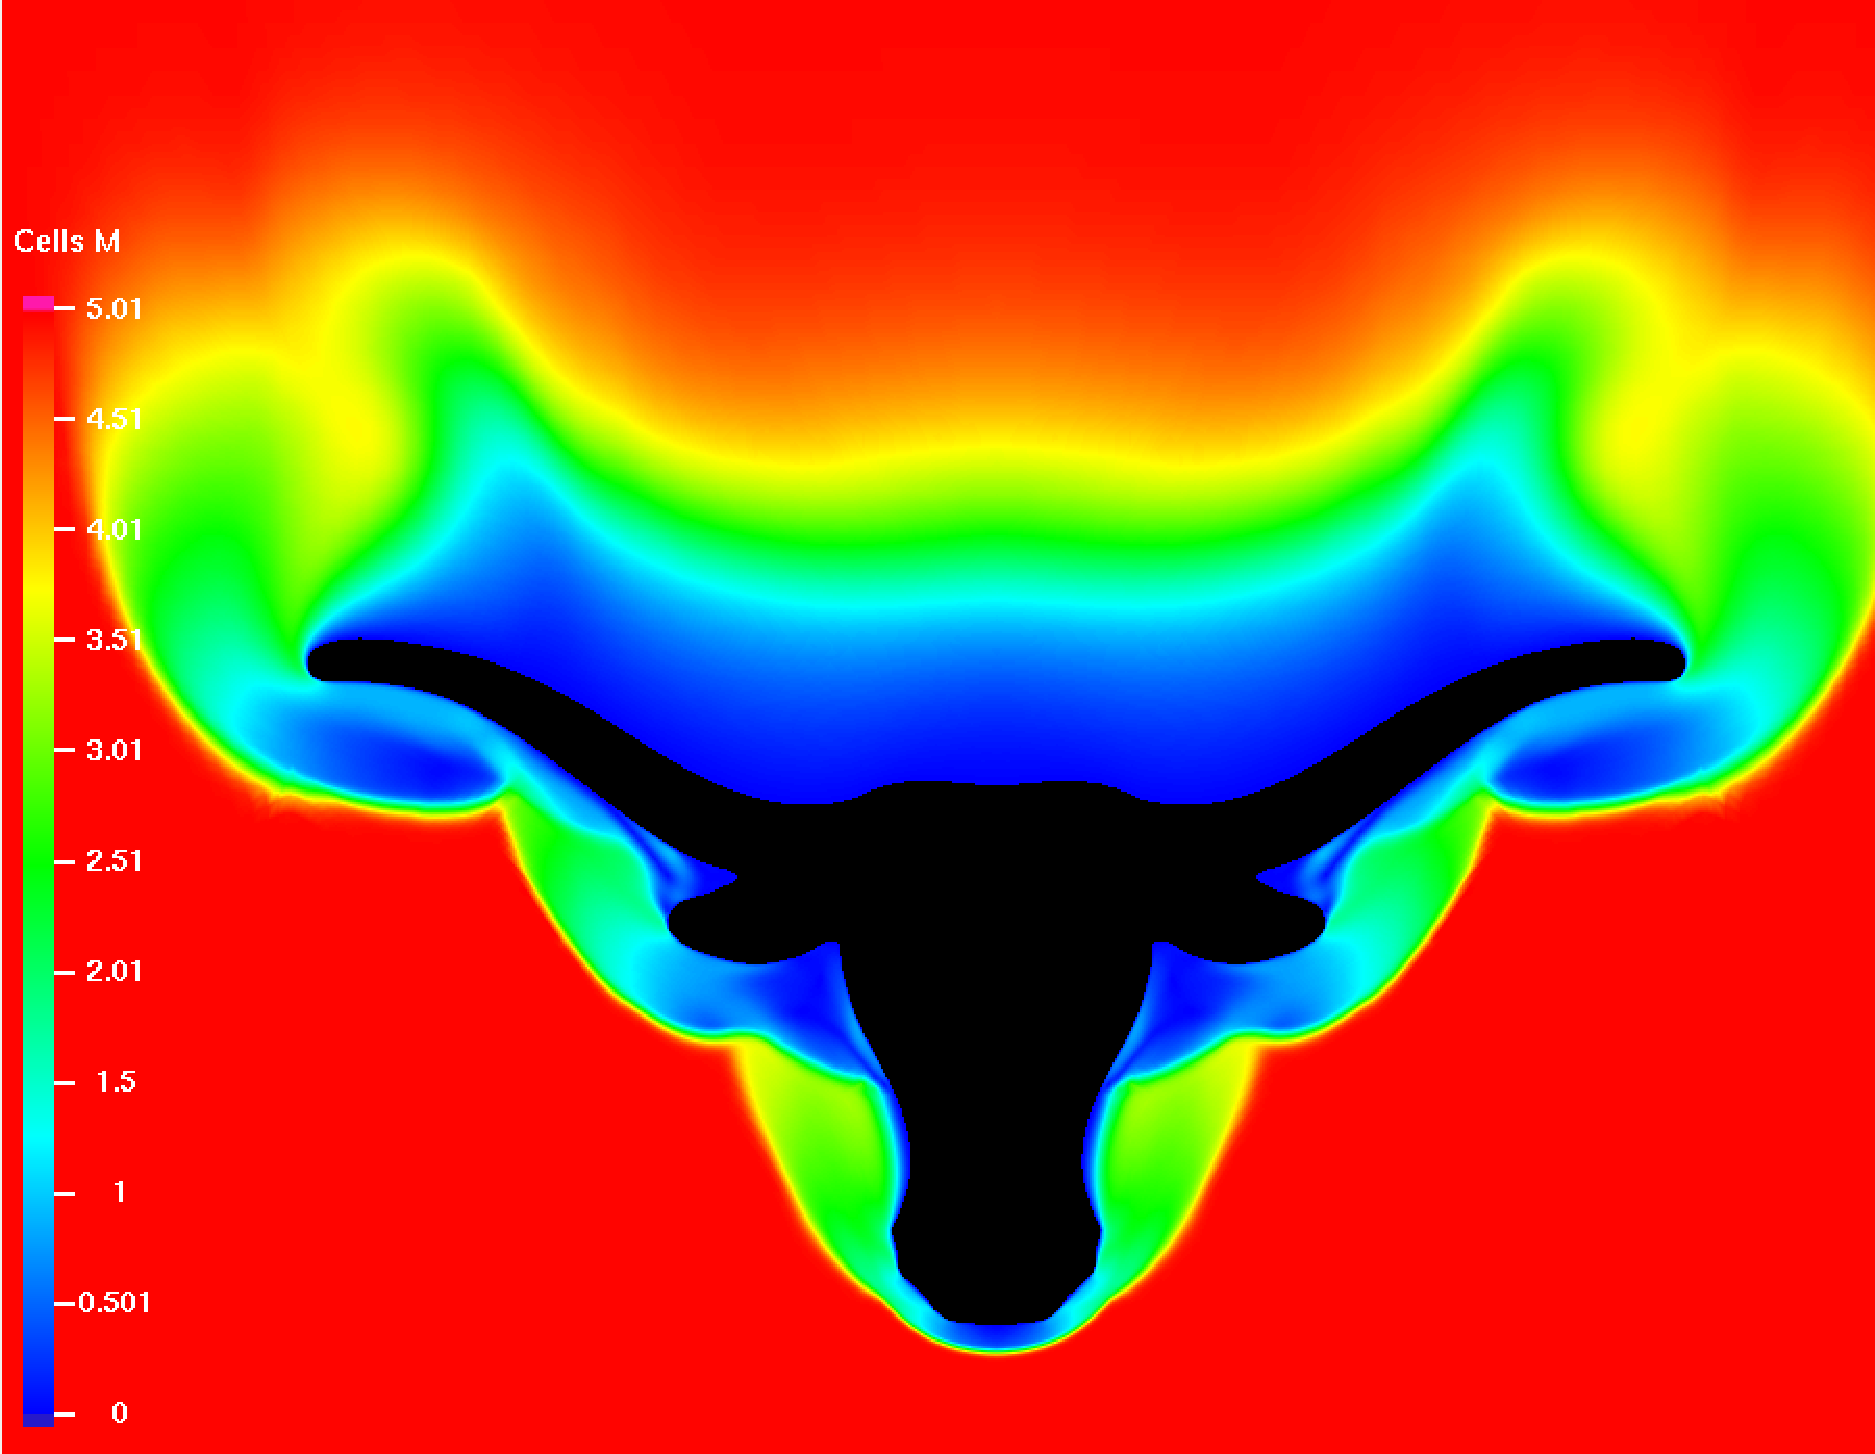
\includegraphics[width=.5\textwidth]{figures/Hypersonic_cow_mach}}
        %\subfigure{\label{fig:fob_adapt_3_sol}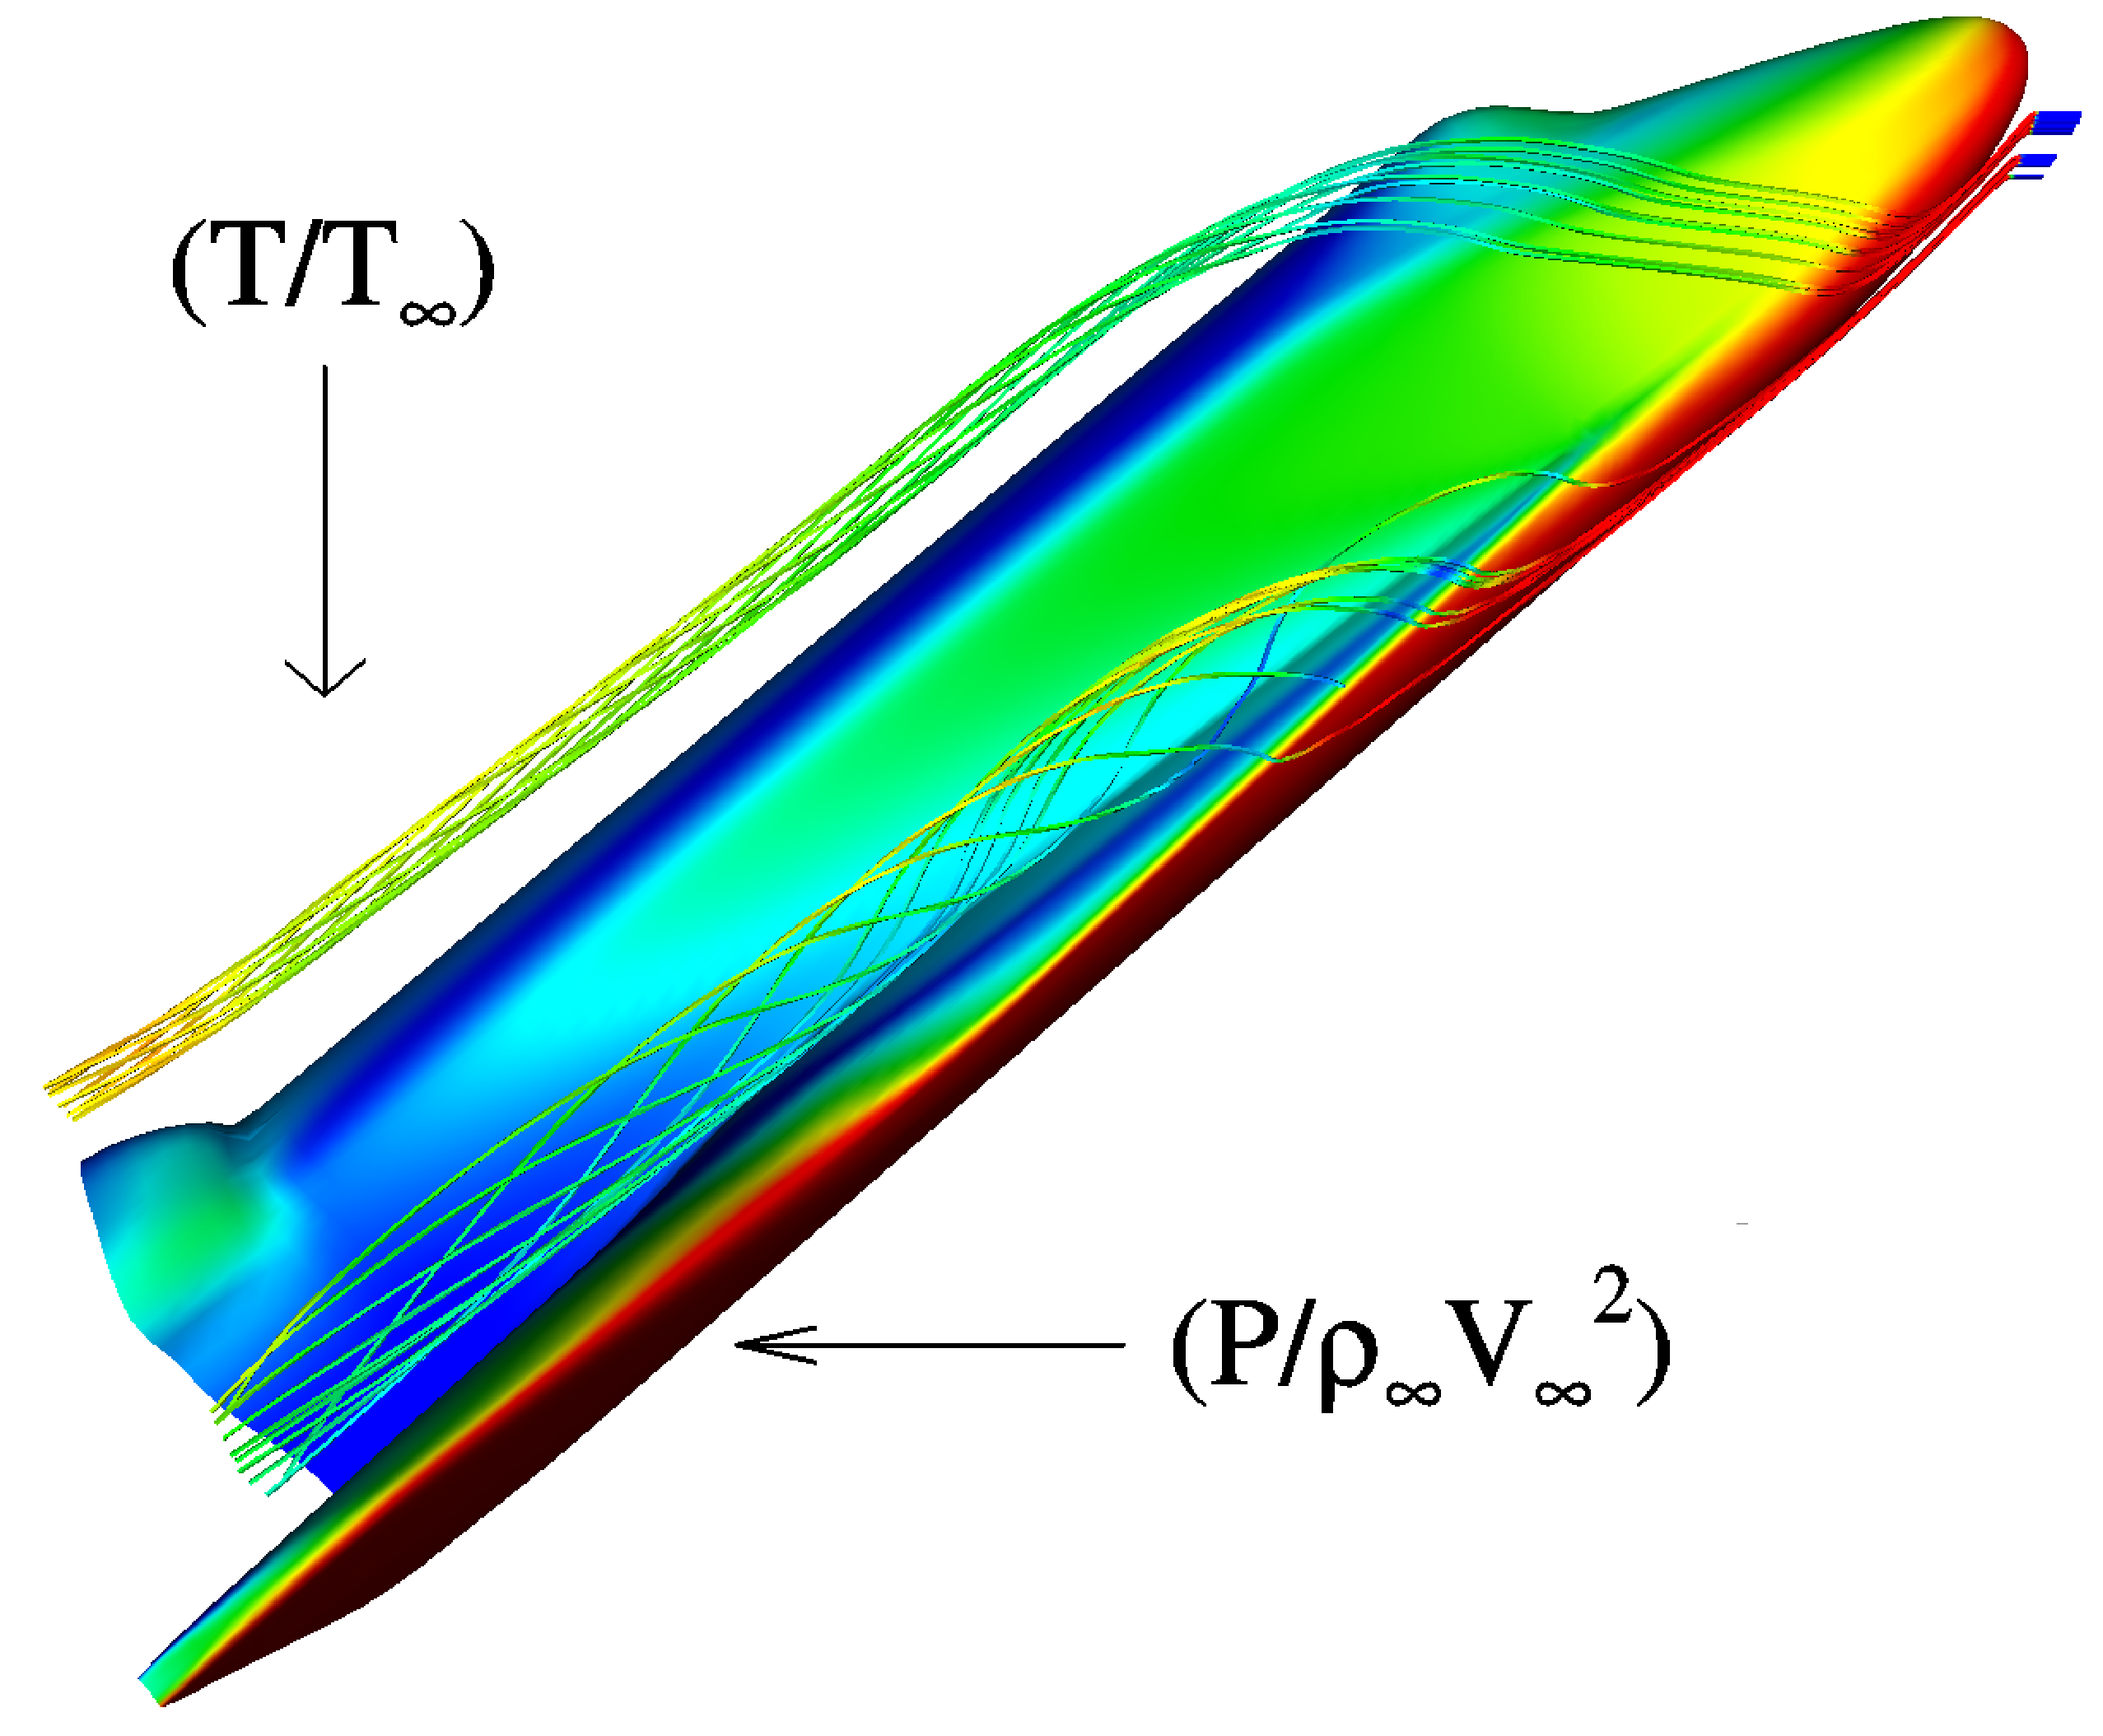
\includegraphics[width=.4\textwidth]{figures/Benkirk_orbiter_reentry_side_view}}
        \subfigure{\label{fig:fob_redist_adapt_10_sol}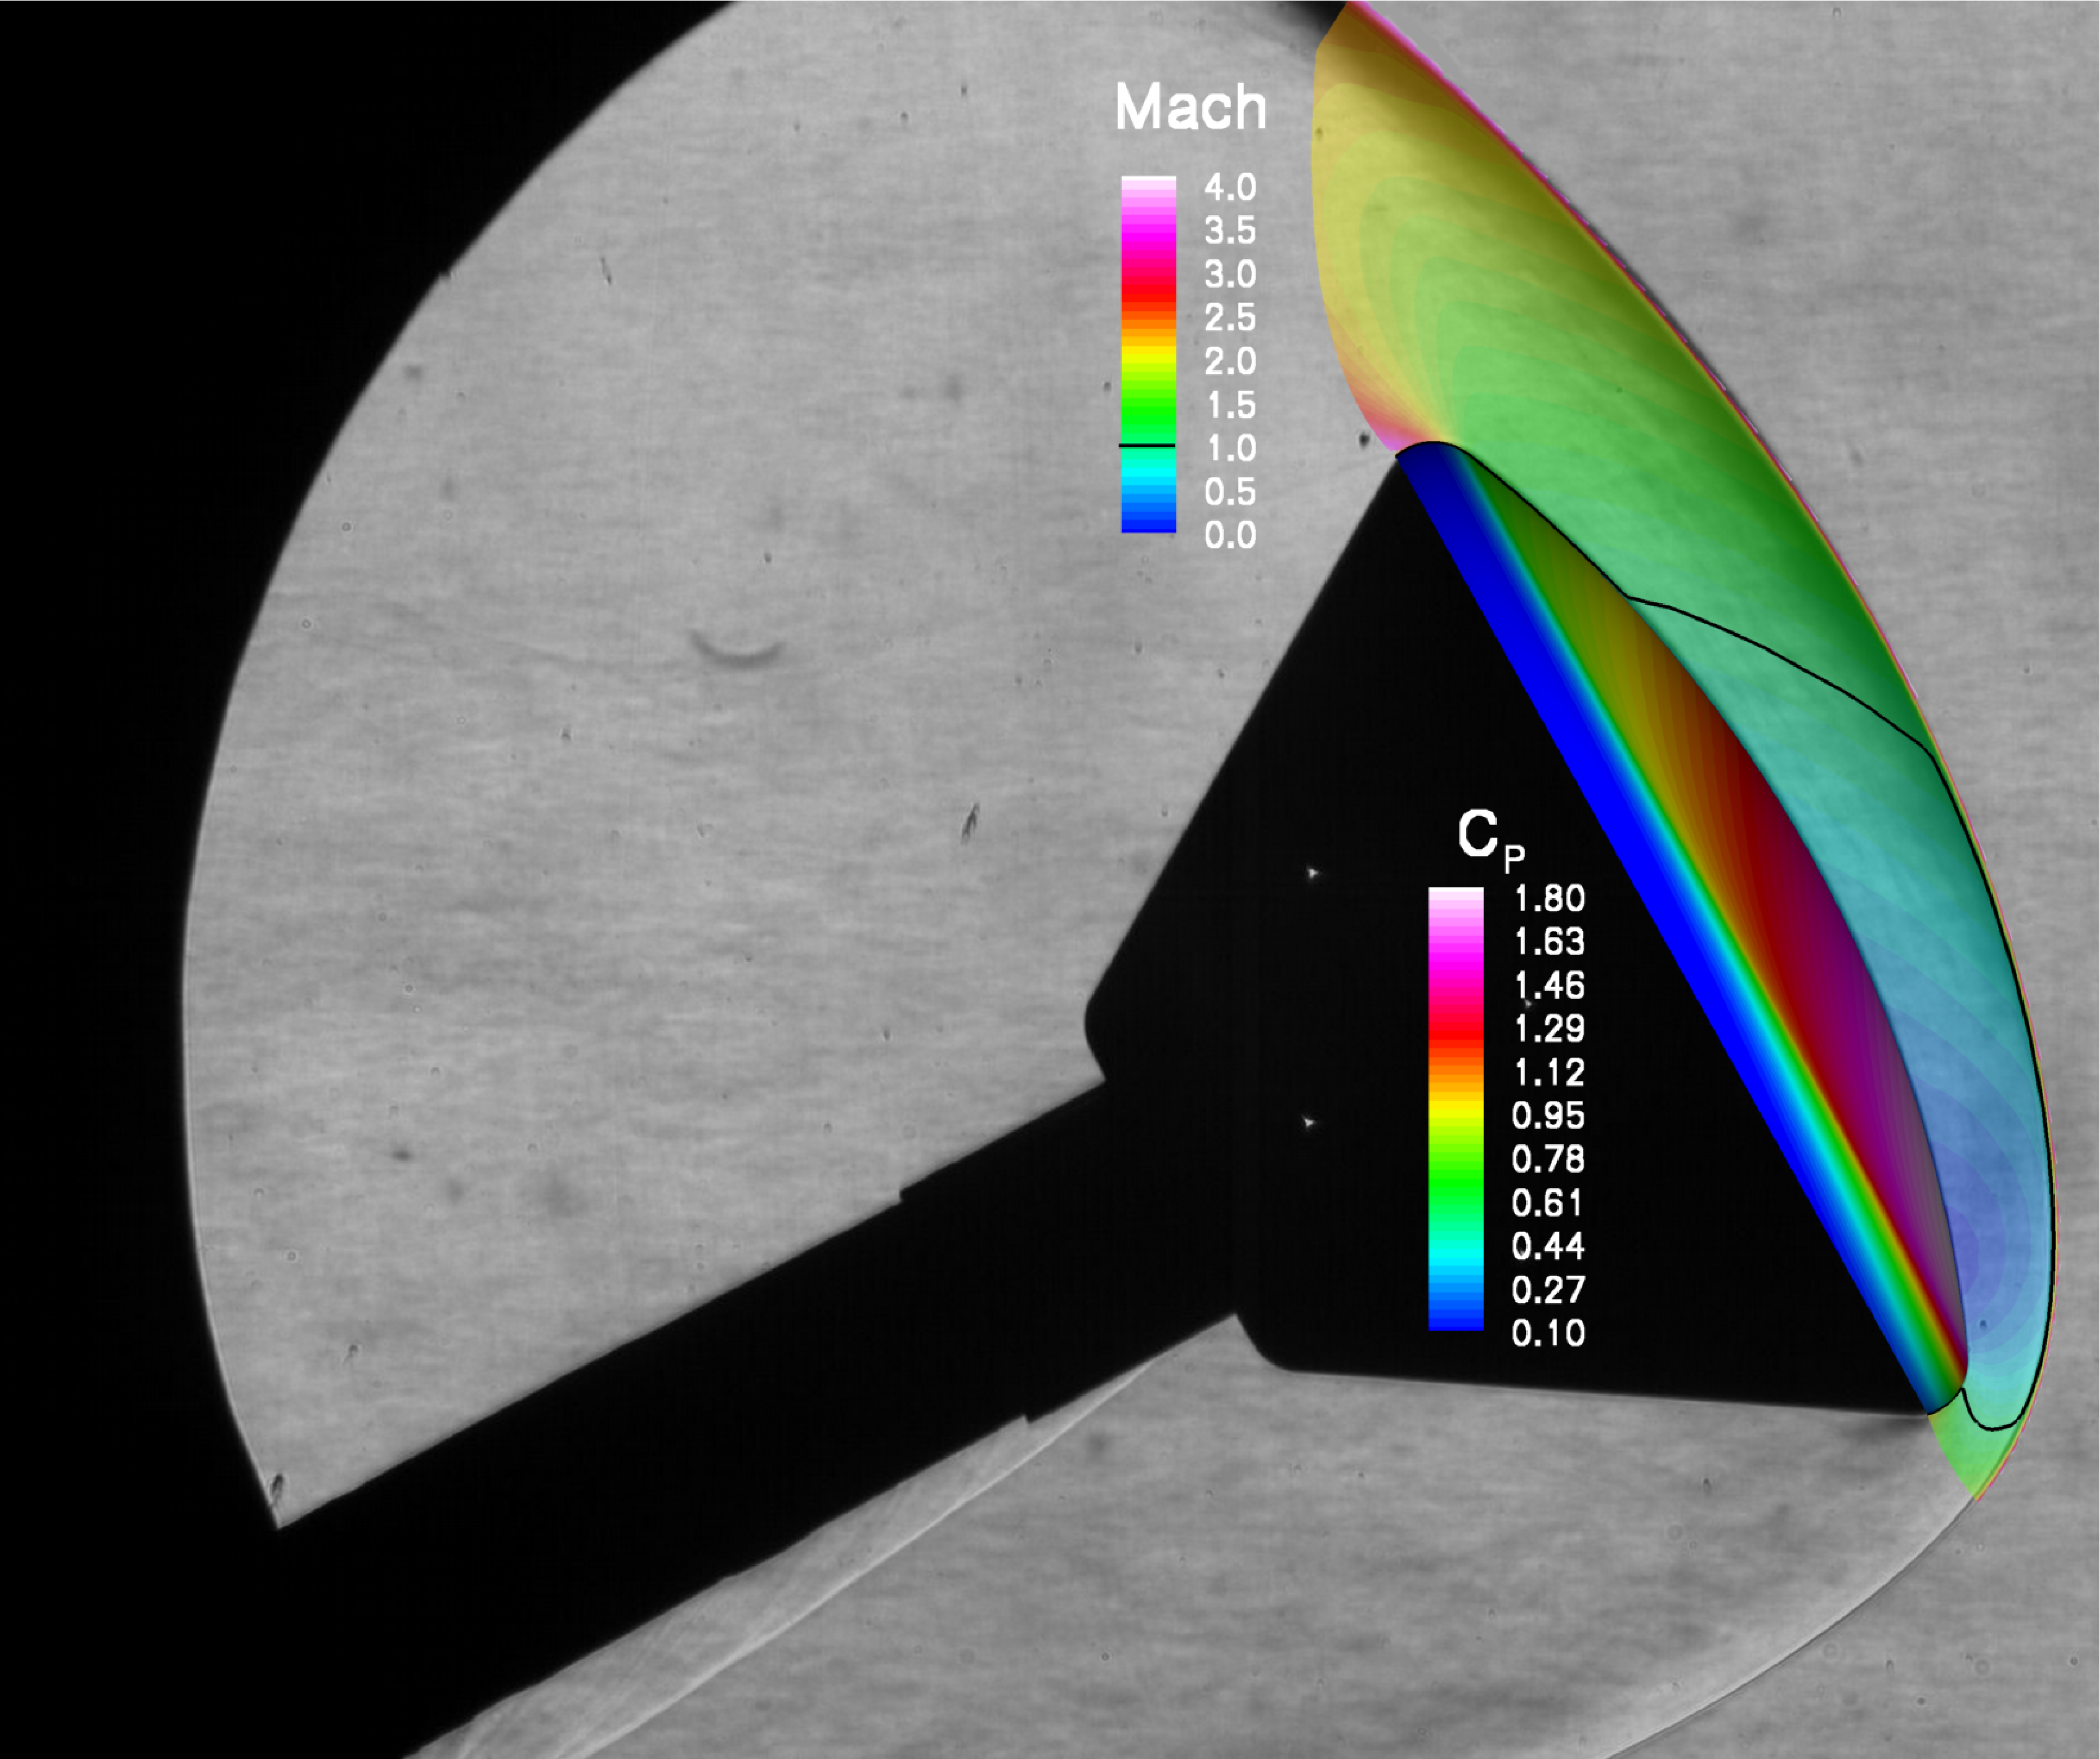
\includegraphics[width=.45\textwidth]{figures/Benkirk_schlieren}}
        %\subfigure{\label{fig:fob_redist_adapt_10_sol}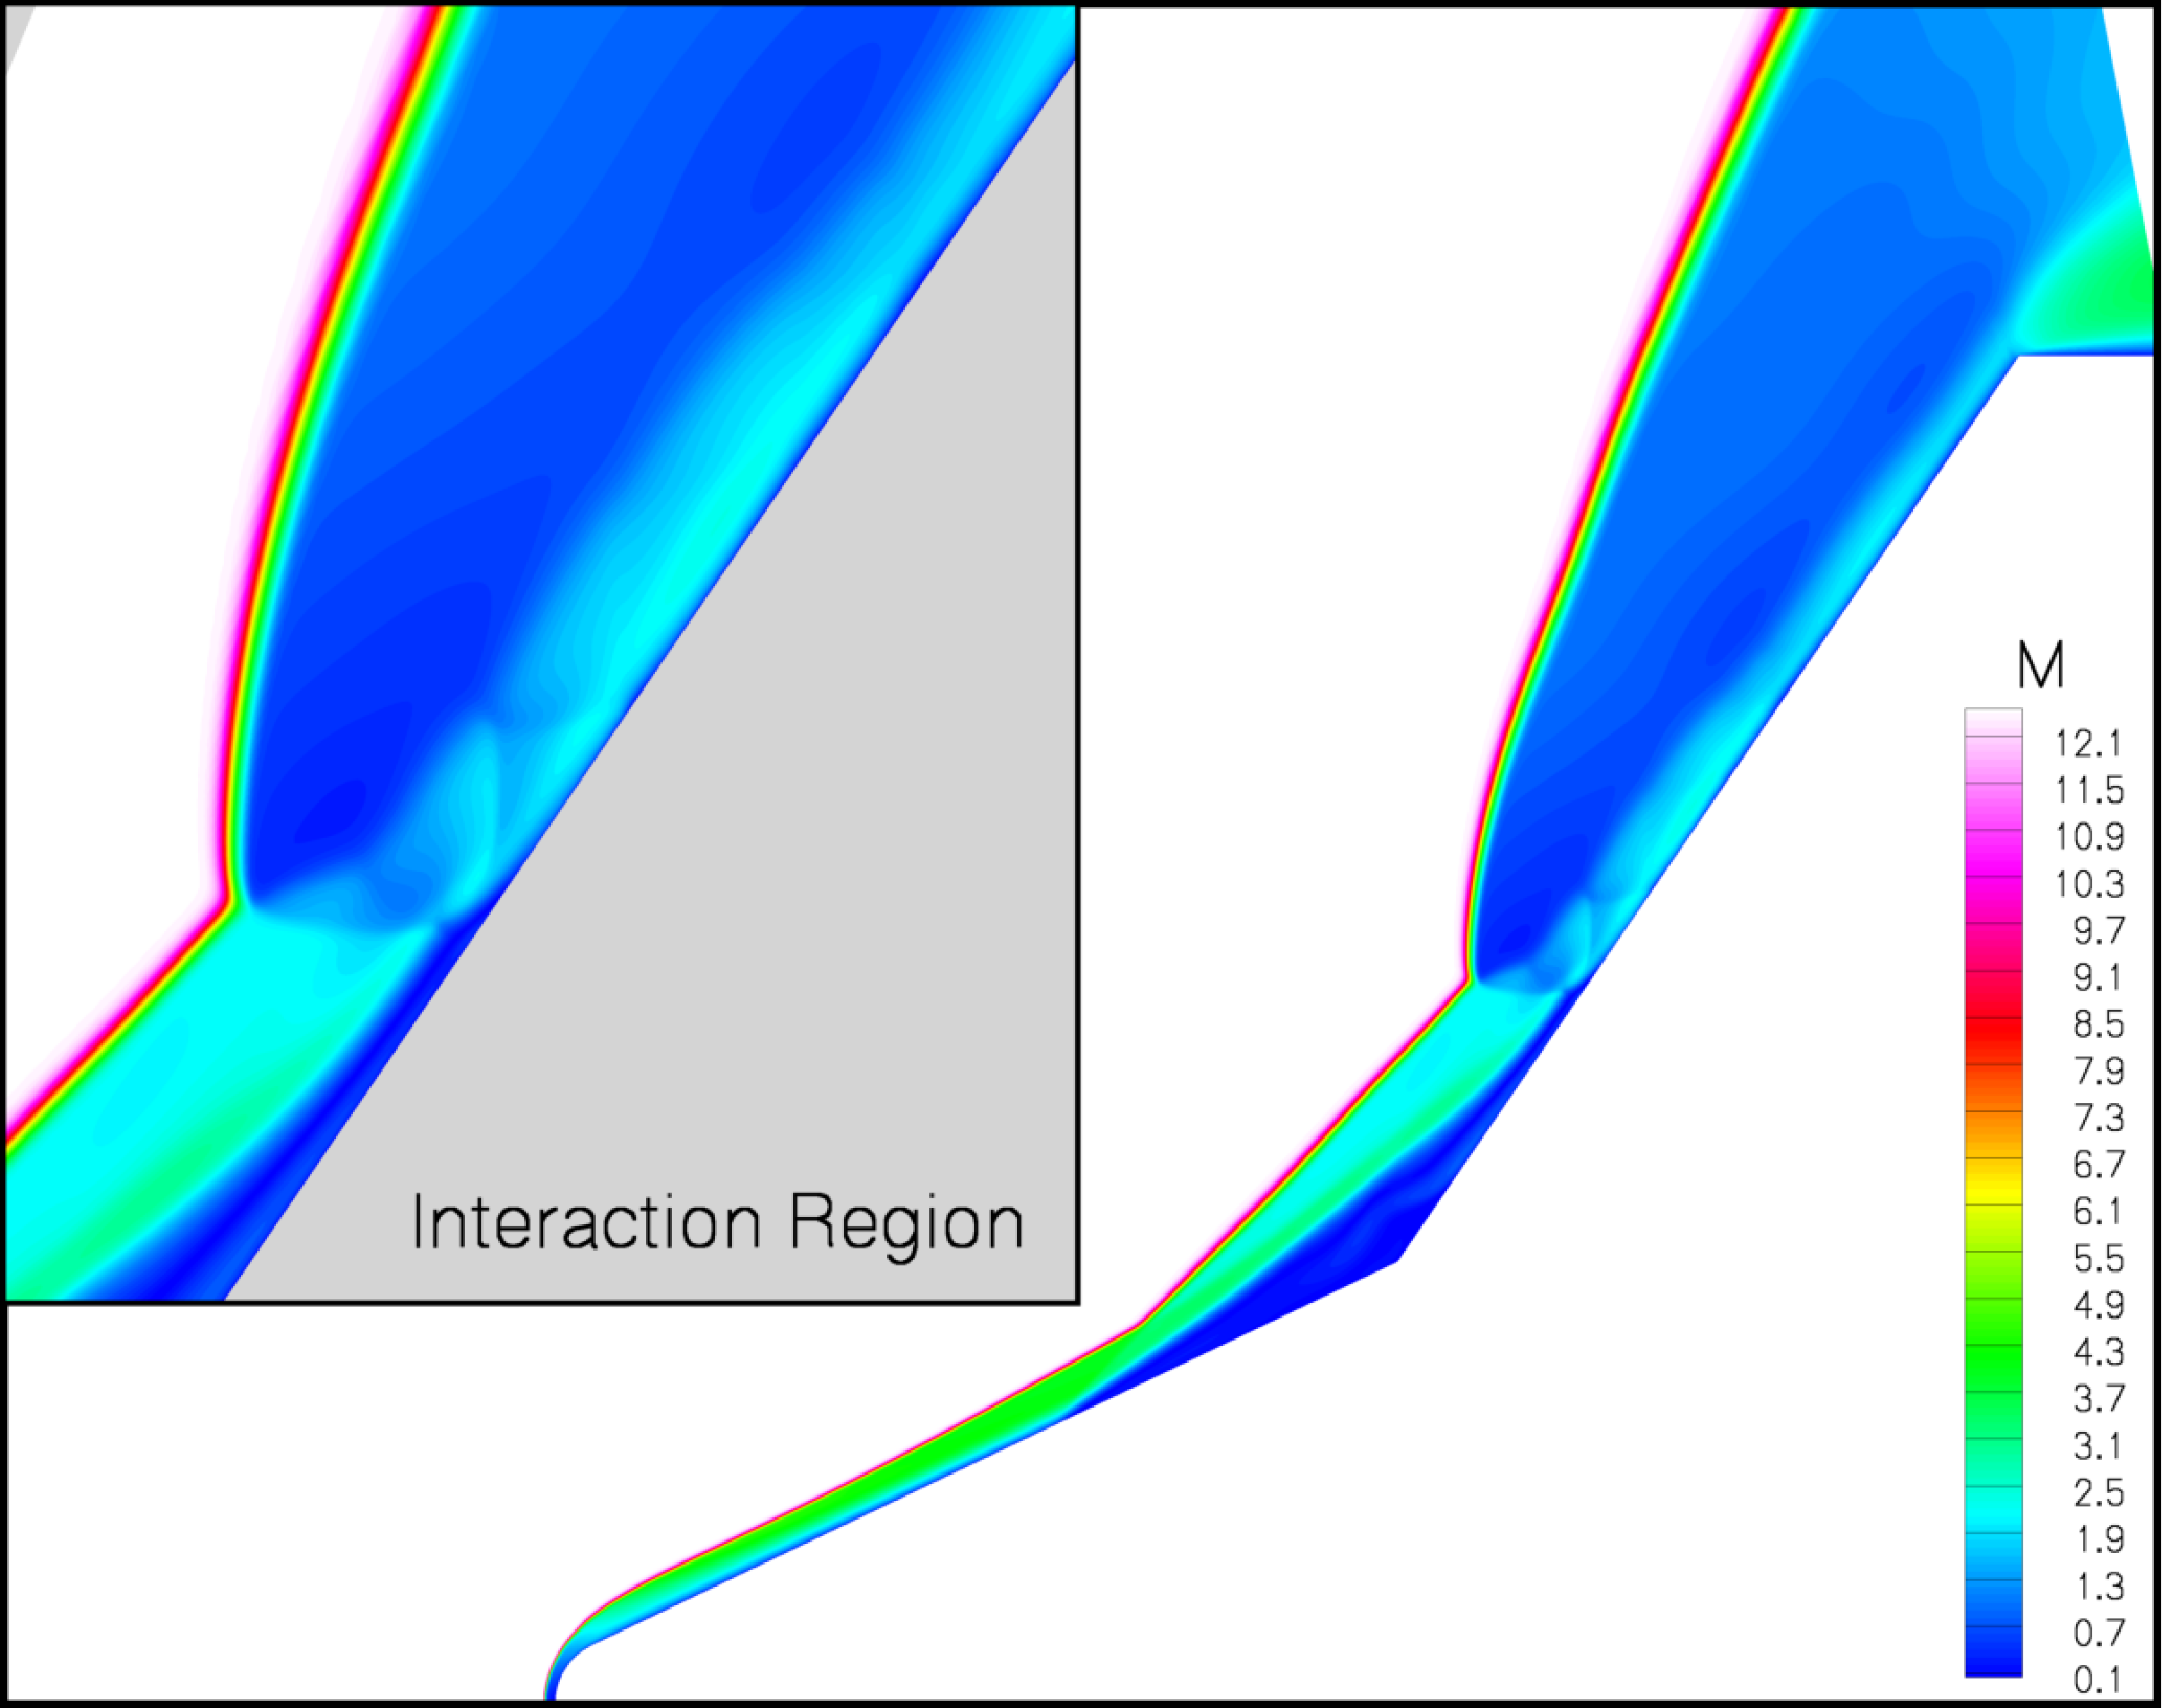
\includegraphics[width=.4\textwidth]{figures/Benkirk_double_cone_M}}
      \end{center}
    \end{figure}
\begin{itemize}
\item {LibMesh is being used in the development of the Orion CEV at NASA.}
\end{itemize}
\end{frame}


\subsection*{Surface-Tension-Driven Flow}
\begin{frame}%[t]
  \begin{center}
    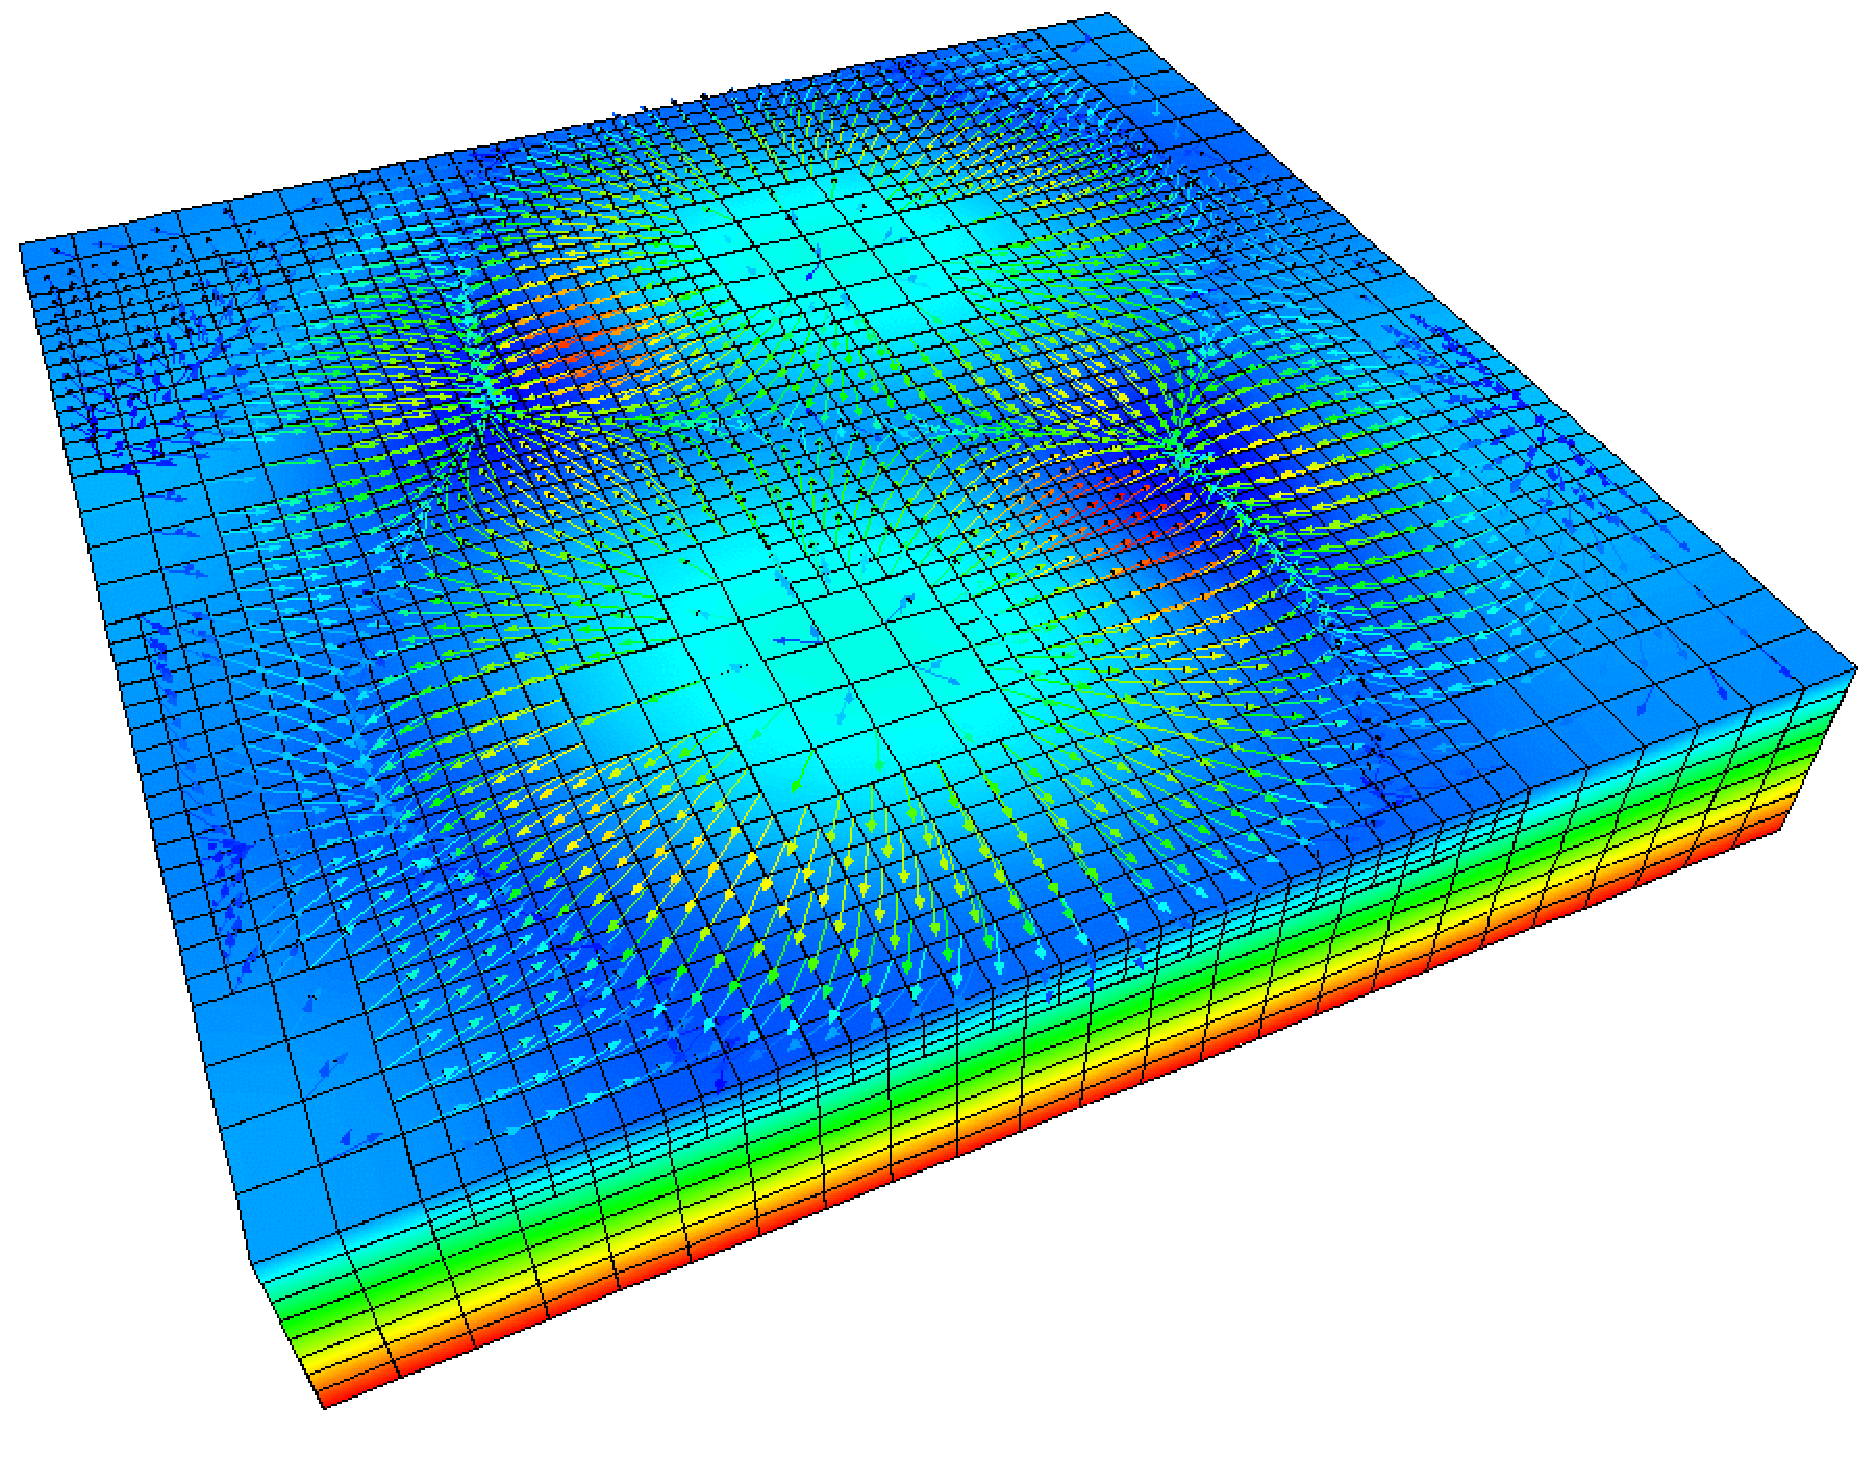
\includegraphics[width=.6\textwidth]{figures/rbm_adapt_soln}    
  \end{center}
  \vspace{-.25in}

%  \begin{block}{}
    \begin{itemize}
    \item{Adaptive grid solution shown
      with temperature contours and velocity vectors.      }
      \end{itemize}
%  \end{block}
\end{frame}


\subsection*{Tumor Angiogenesis}
\begin{frame}[t]
  \begin{center}
    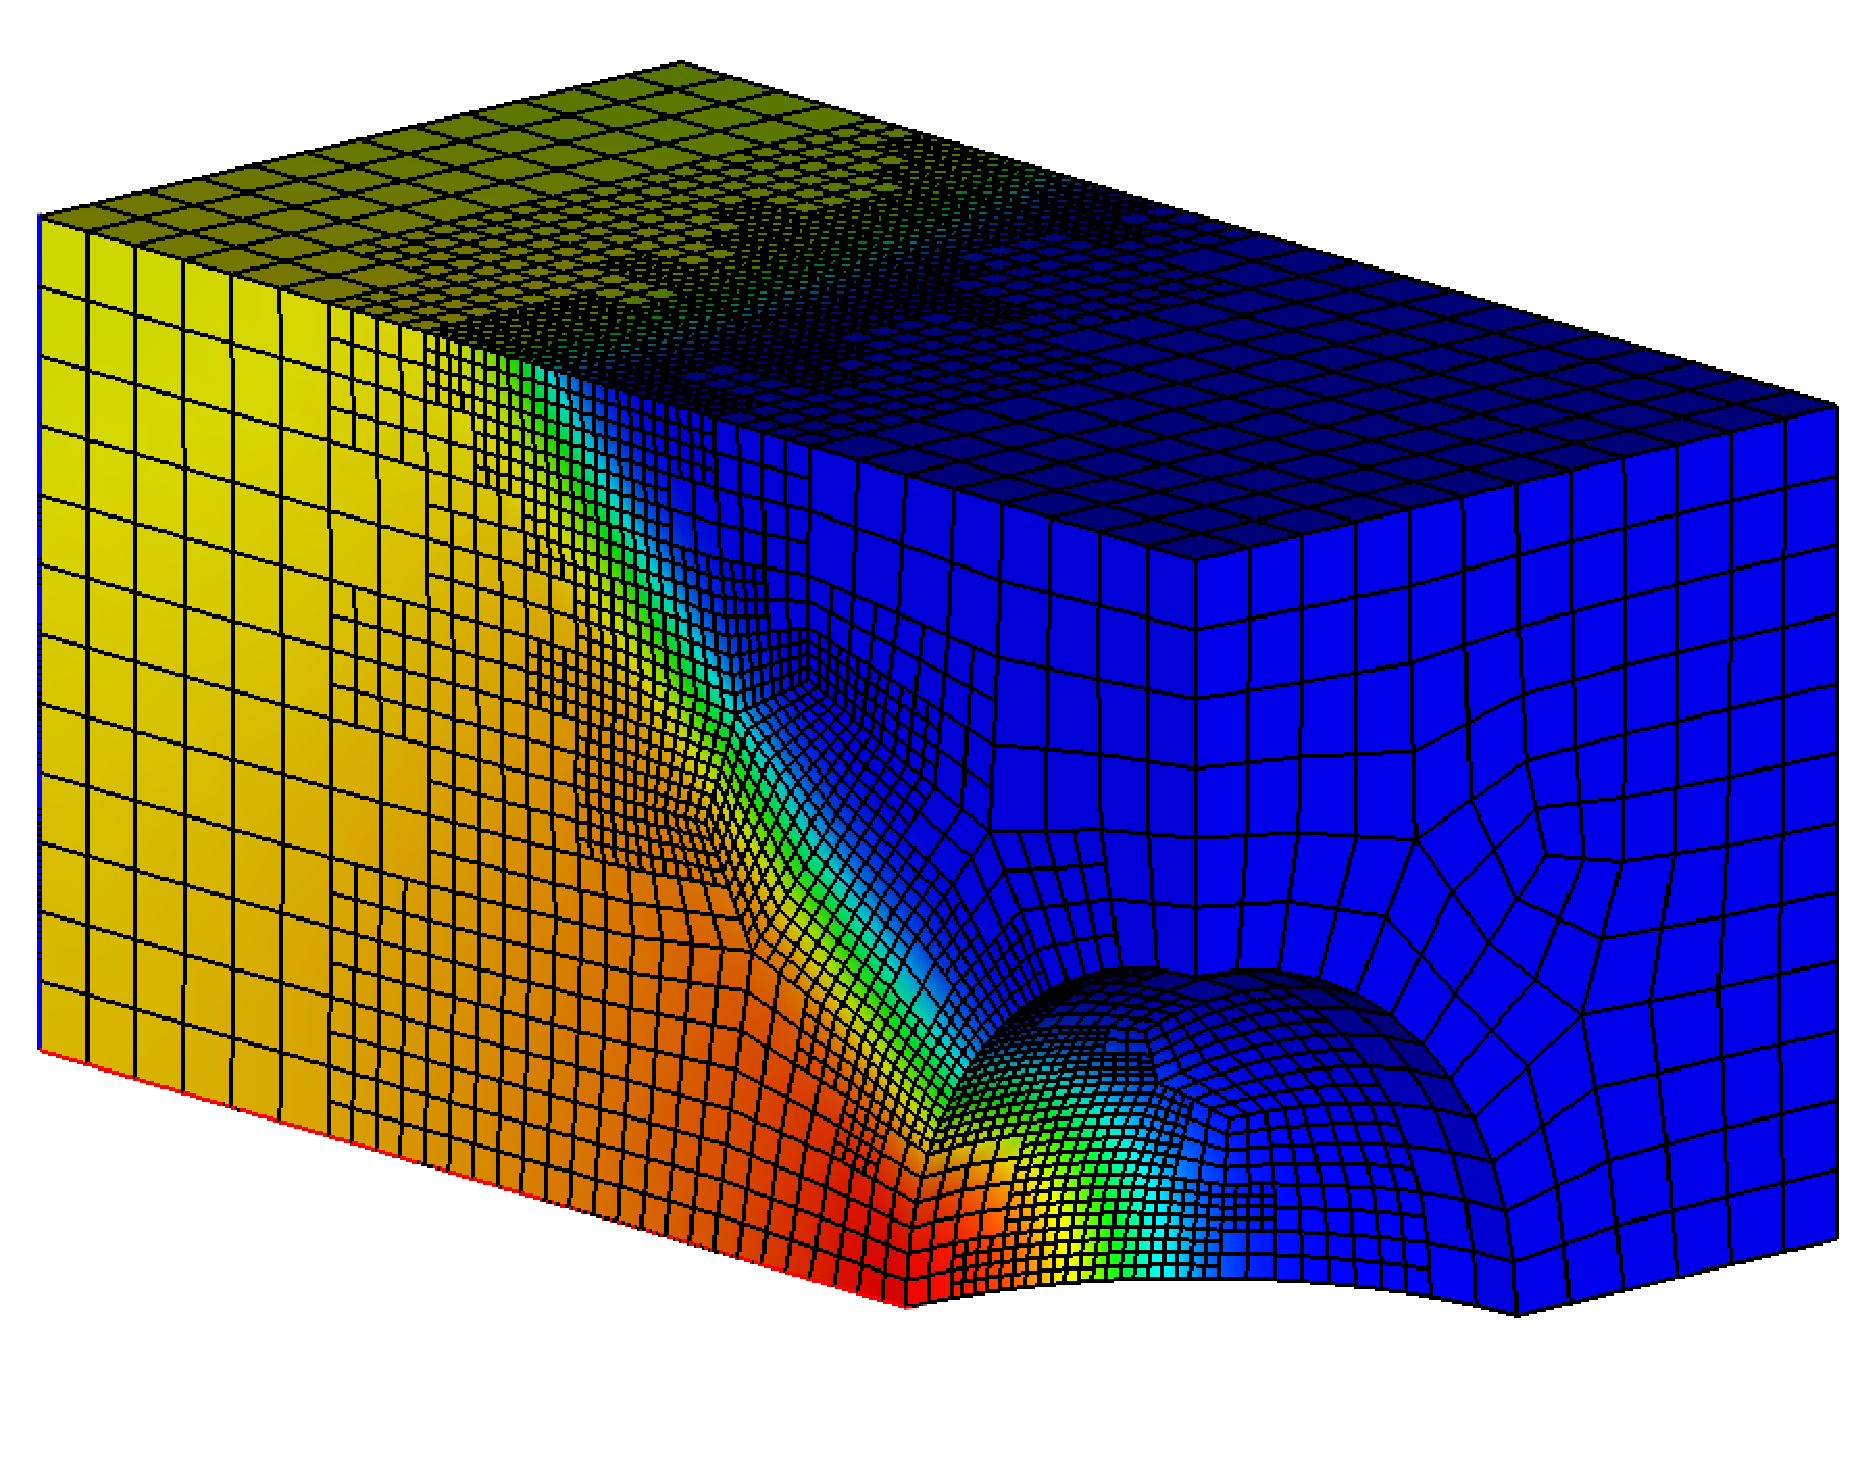
\includegraphics[width=.6\textwidth]{figures/tumor_model}    
  \end{center}
\vspace{-.35in}
%%   \begin{block}{}
    \begin{itemize}
    \item{A sharp advancing endothelial cell front approaches the
      tumor, eventually inducing blood vessel formation.      }
      \end{itemize}
%%   \end{block}
\end{frame}

\subsection*{Cahn-Hilliard Phase Separation}
\begin{frame}
\begin{center}
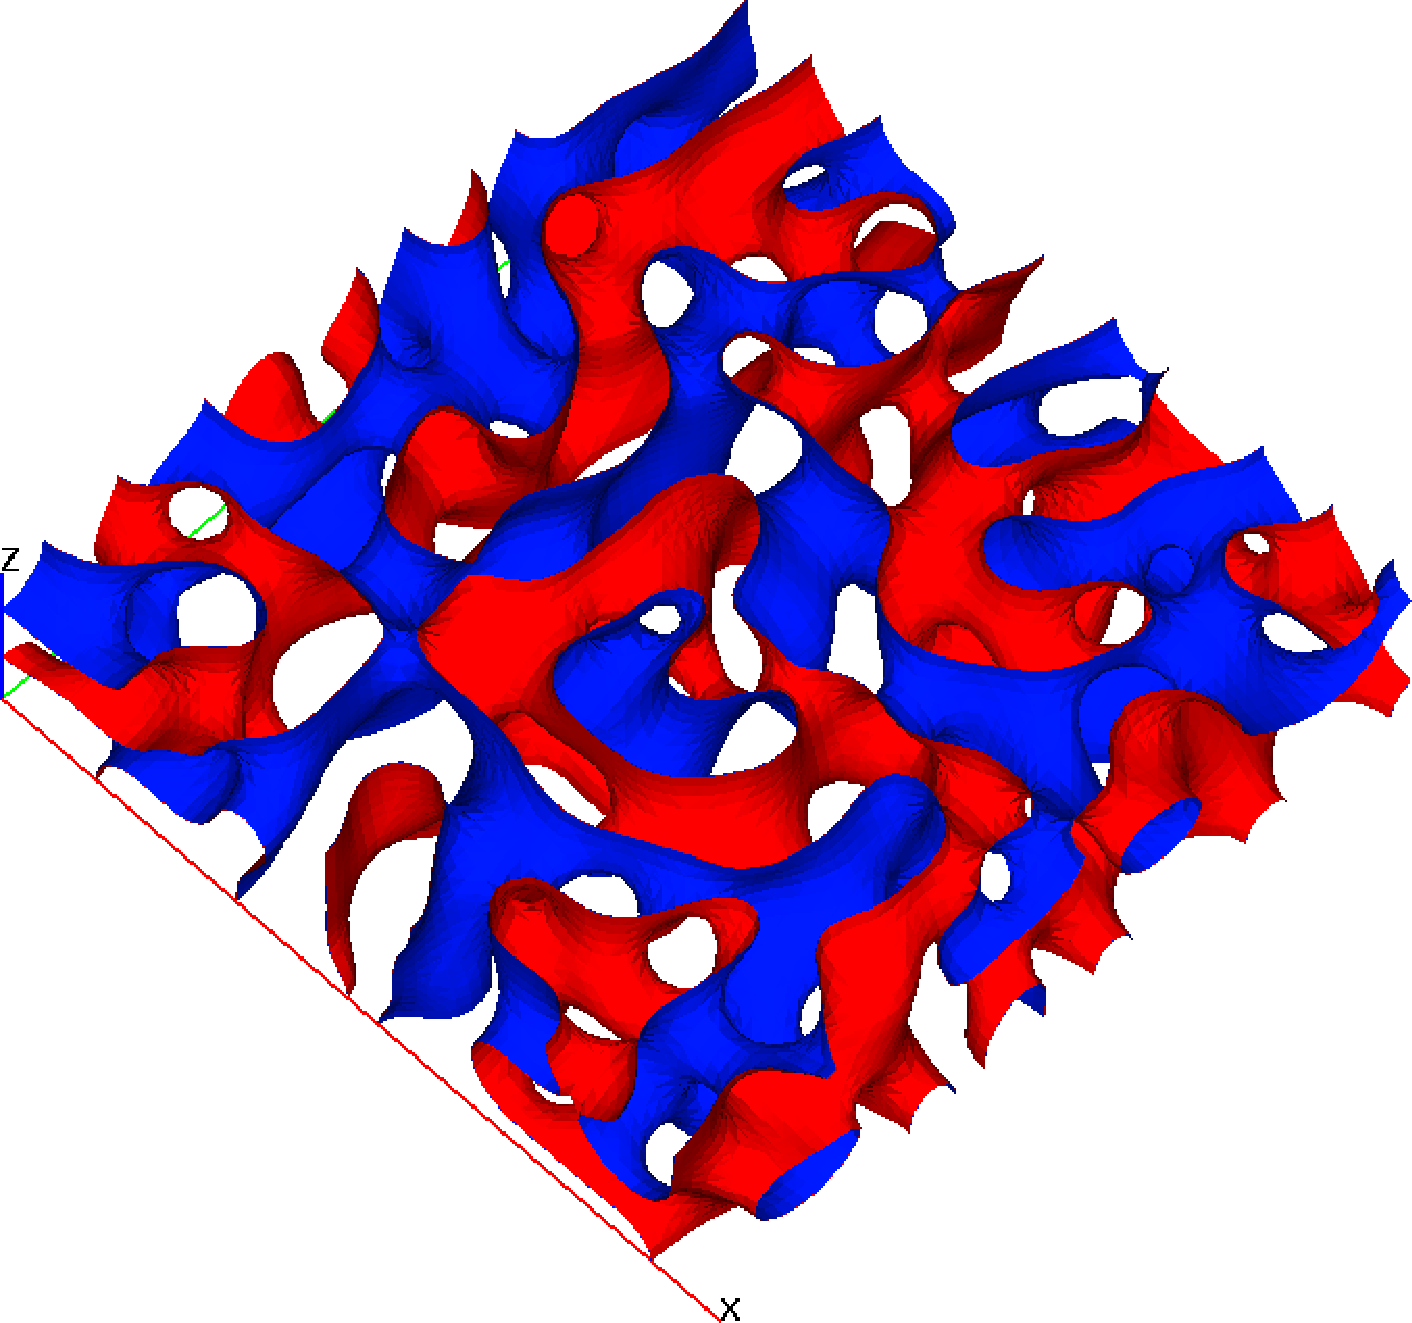
\includegraphics[width=.3\textwidth]{figures/ch3D02-048}
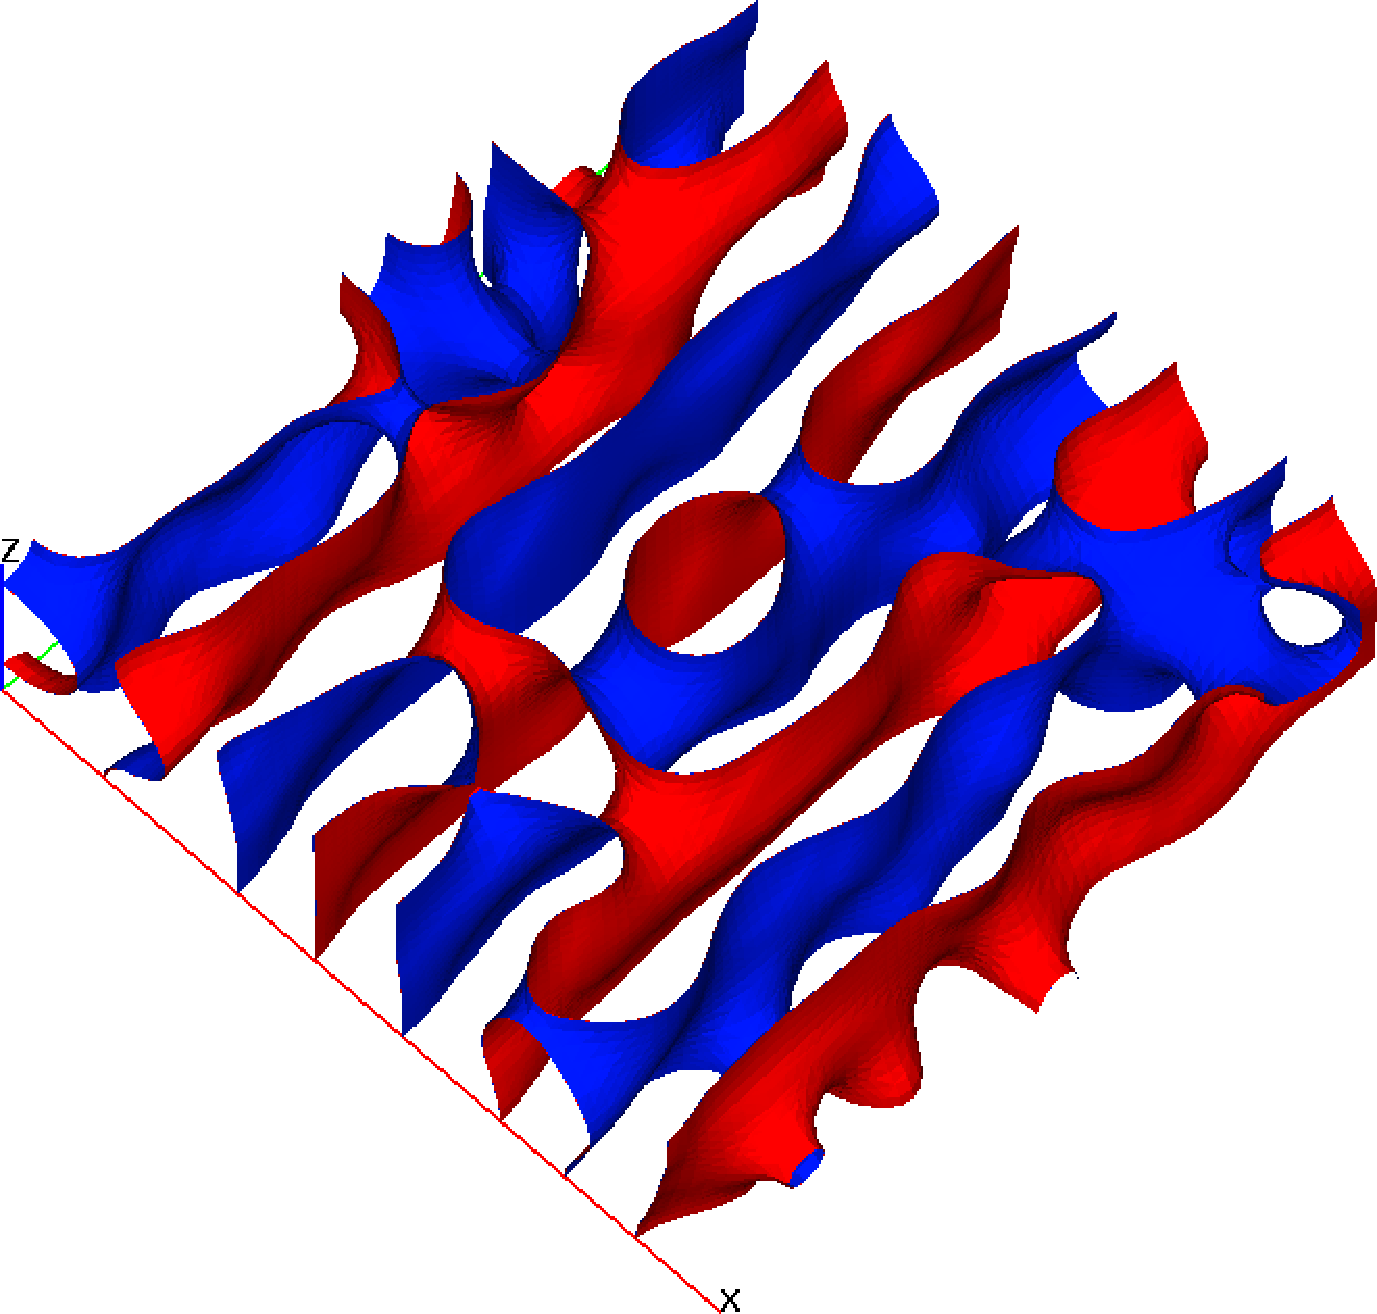
\includegraphics[width=.3\textwidth]{figures/ch3D02-096}
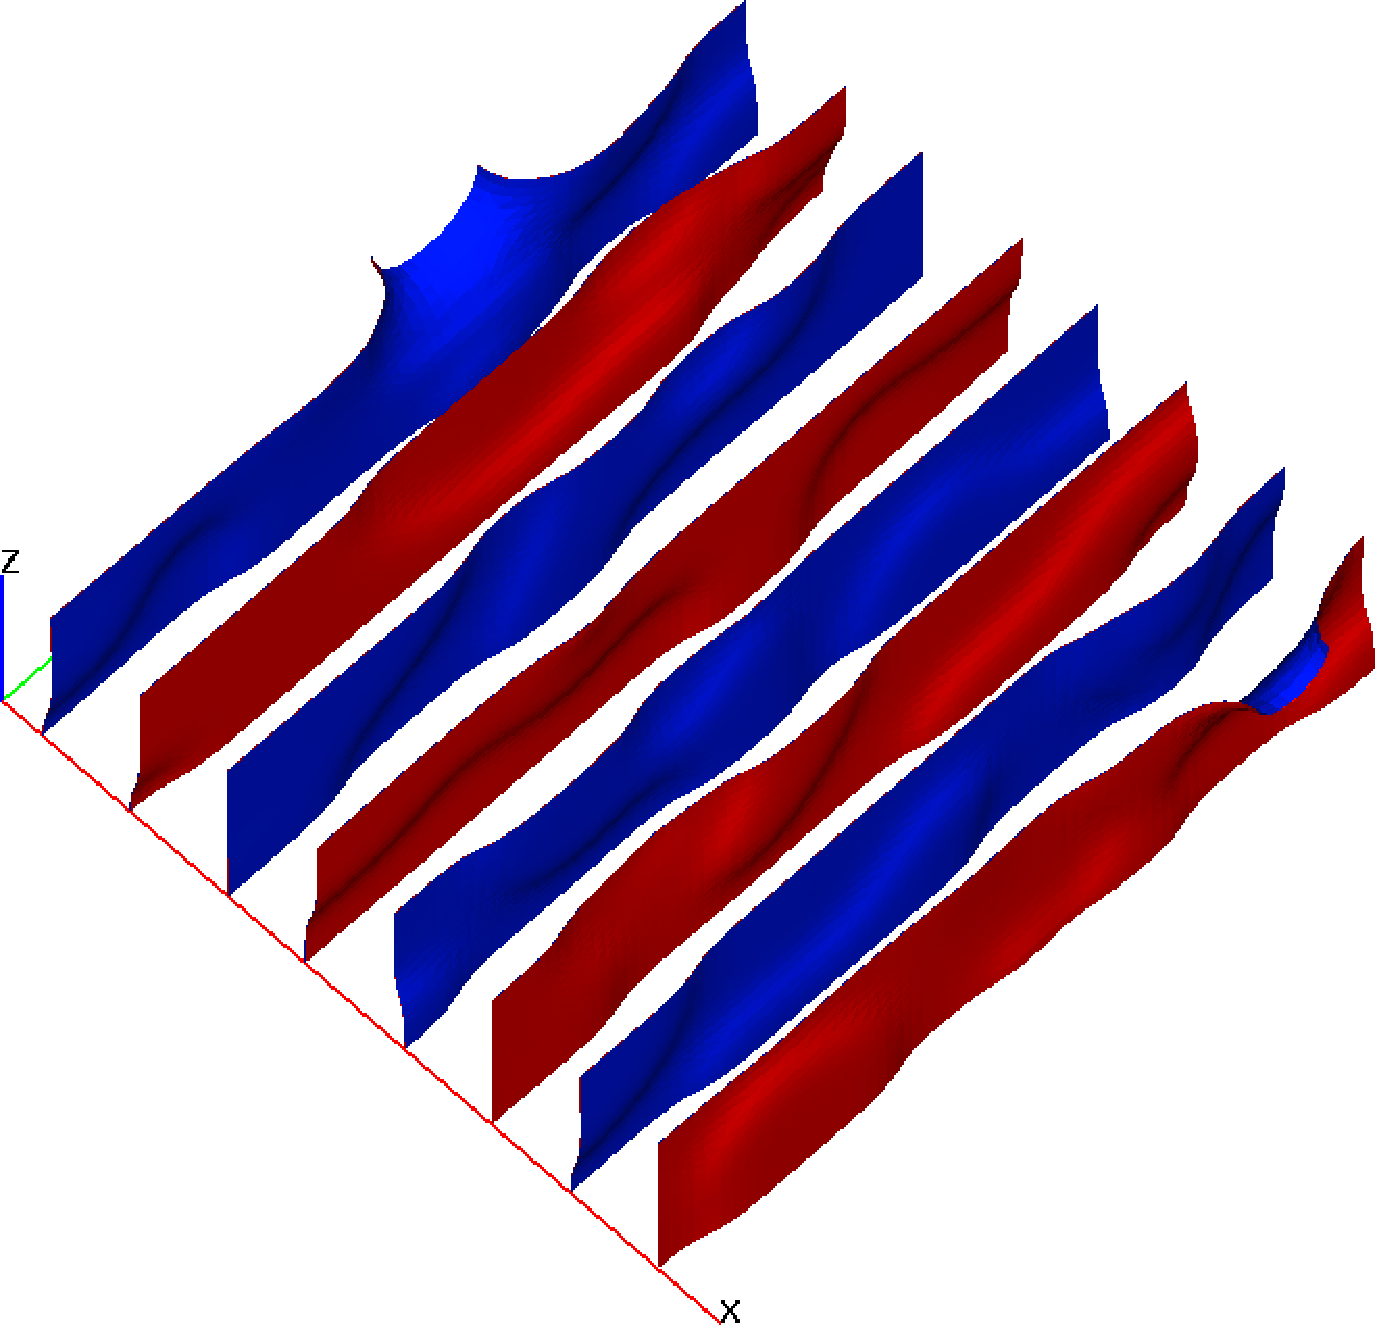
\includegraphics[width=.3\textwidth]{figures/ch3D02-192}
\end{center}
\begin{itemize}
\item Single-phase regions gradually coalesce
%\item Motion into curvature vector resembles surface tension
\item Patterning may occur when additional stresses are present
\end{itemize}
\end{frame}

\section*{Reference}
\begin{frame}[t]
  \begin{block}{}
    \begin{itemize}
    \item{
      %Some applications are shown from:
      %\\
      %\vspace{.5in}
      %\begin{block}{}
      B. Kirk, J. Peterson, R. Stogner and G. Carey, ``libMesh: a C++
      library for parallel adaptive mesh refinement/coarsening
      simulations'',  \emph{Engineering with Computers}, vol.~22, no.~3--4, p.~237--254, 2006.
      %\end{block}
      }
    \item{
      Public site, mailing lists, SVN tree, examples, etc.:
\texttt{http://libmesh.sf.net/}
      }
    \end{itemize}
  \end{block}
\end{frame}


\subsection*{How many people use LibMesh?}
\begin{frame}[t]
\begin{center}
    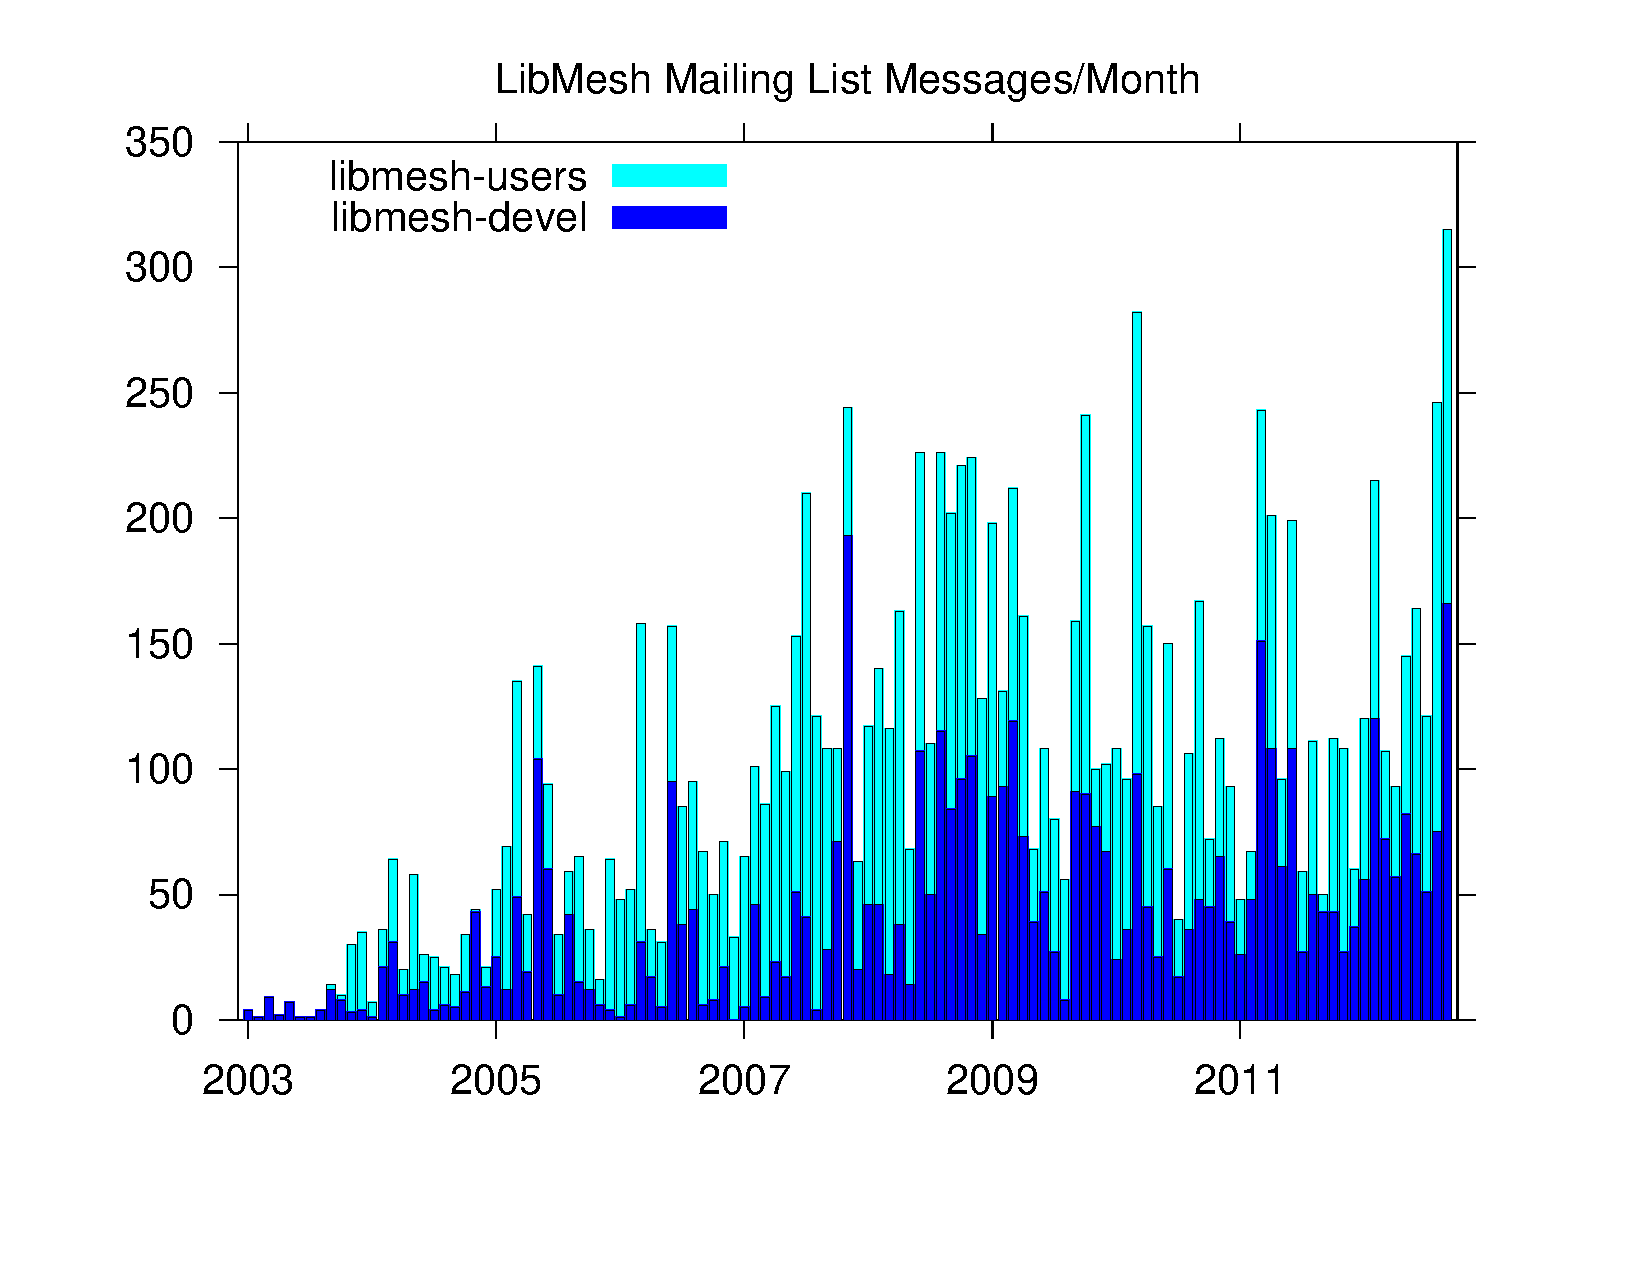
\includegraphics[viewport=55 50 760 560,
    clip=true,width=.95\textwidth]{figures/libmesh_mailinglists}
  %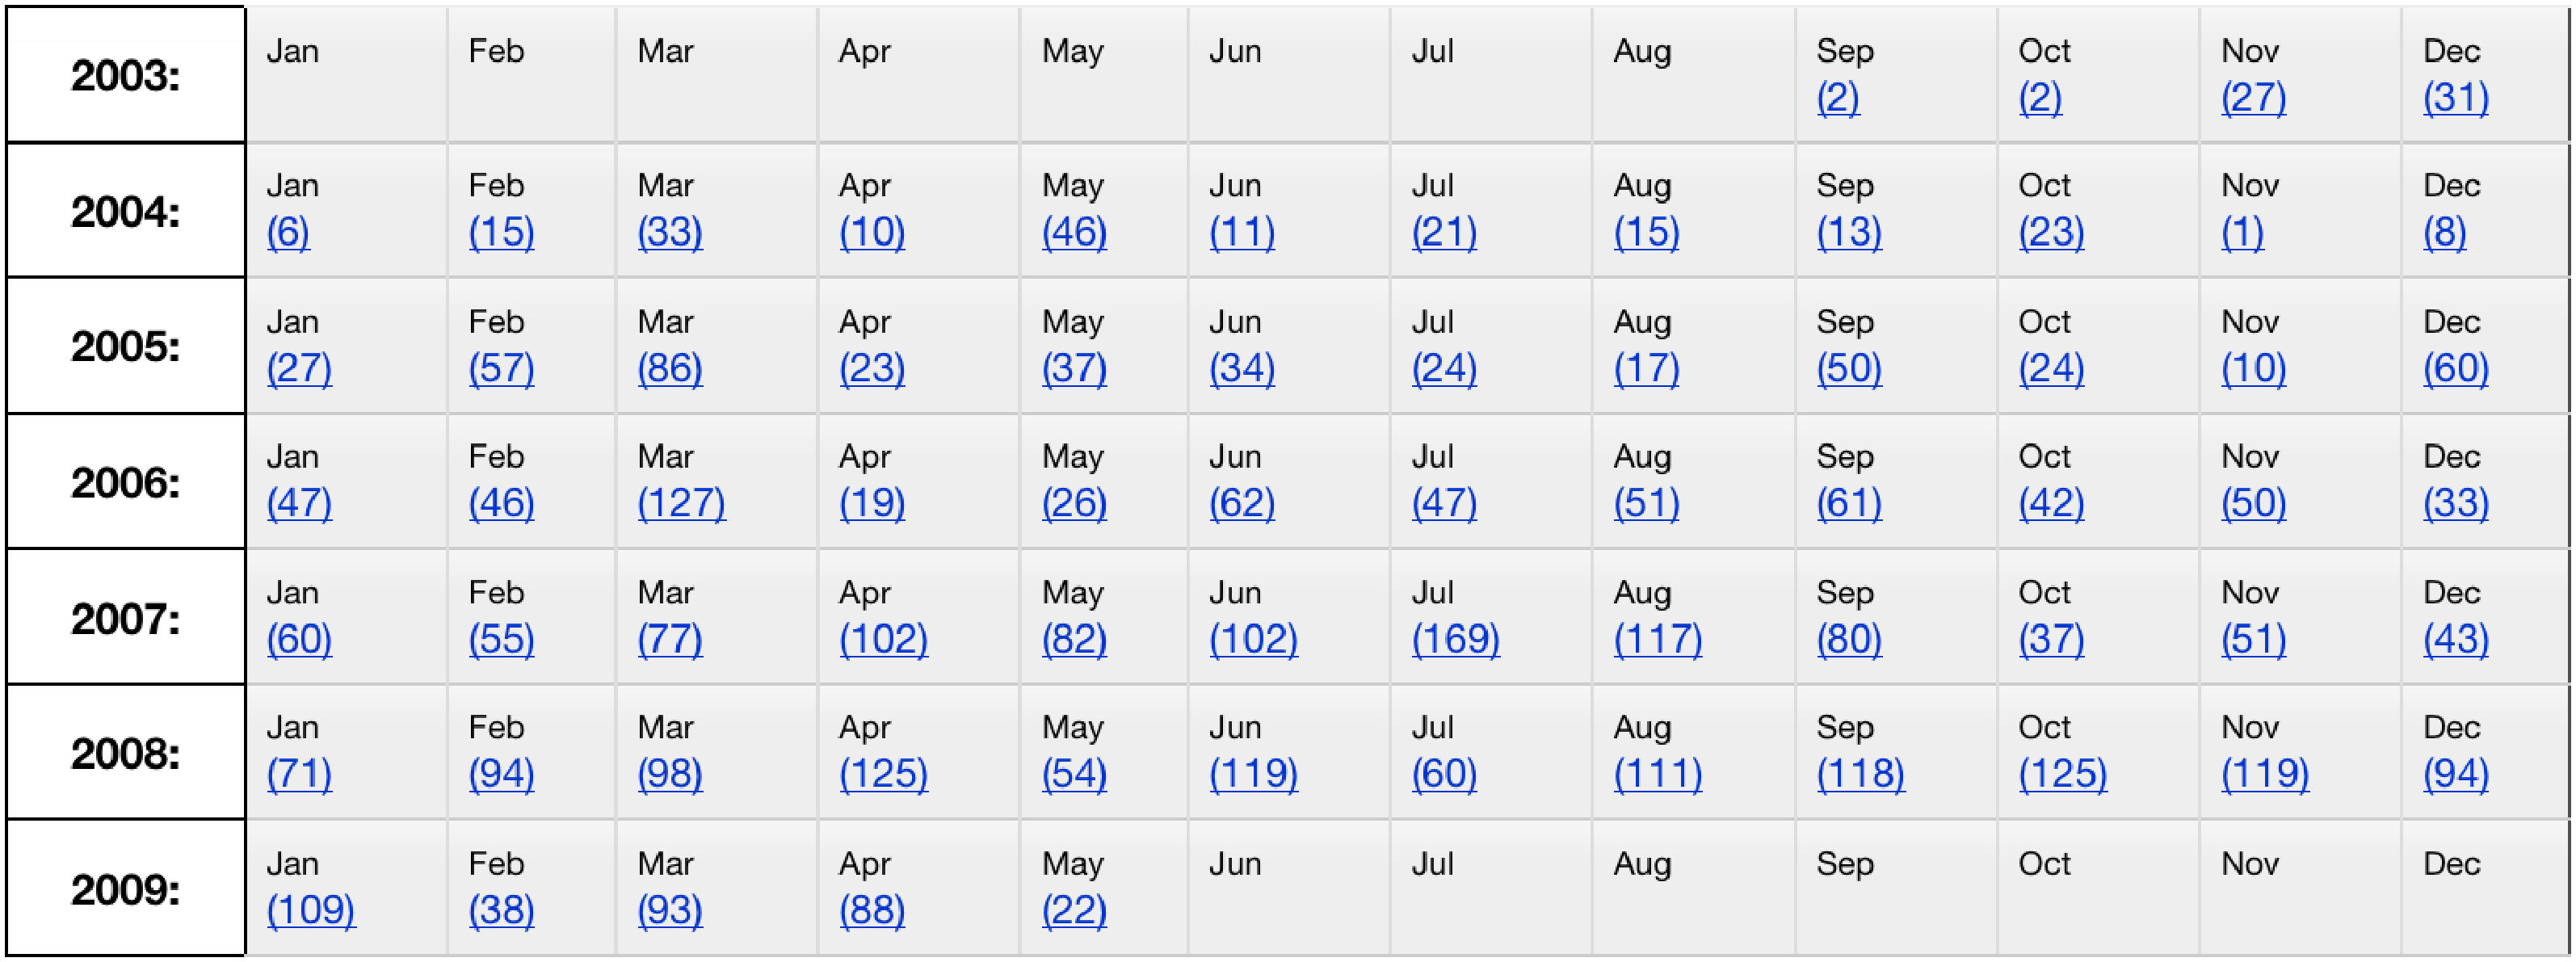
\includegraphics[width=1\textwidth]{figures/libmesh_users_msg_count_big}
\end{center}
%   \begin{itemize}
%   \item {Messages to the libmesh-users mailing list.}
%   \end{itemize}
\end{frame}

\begin{frame}[t]
\begin{center}
  %\fbox{
    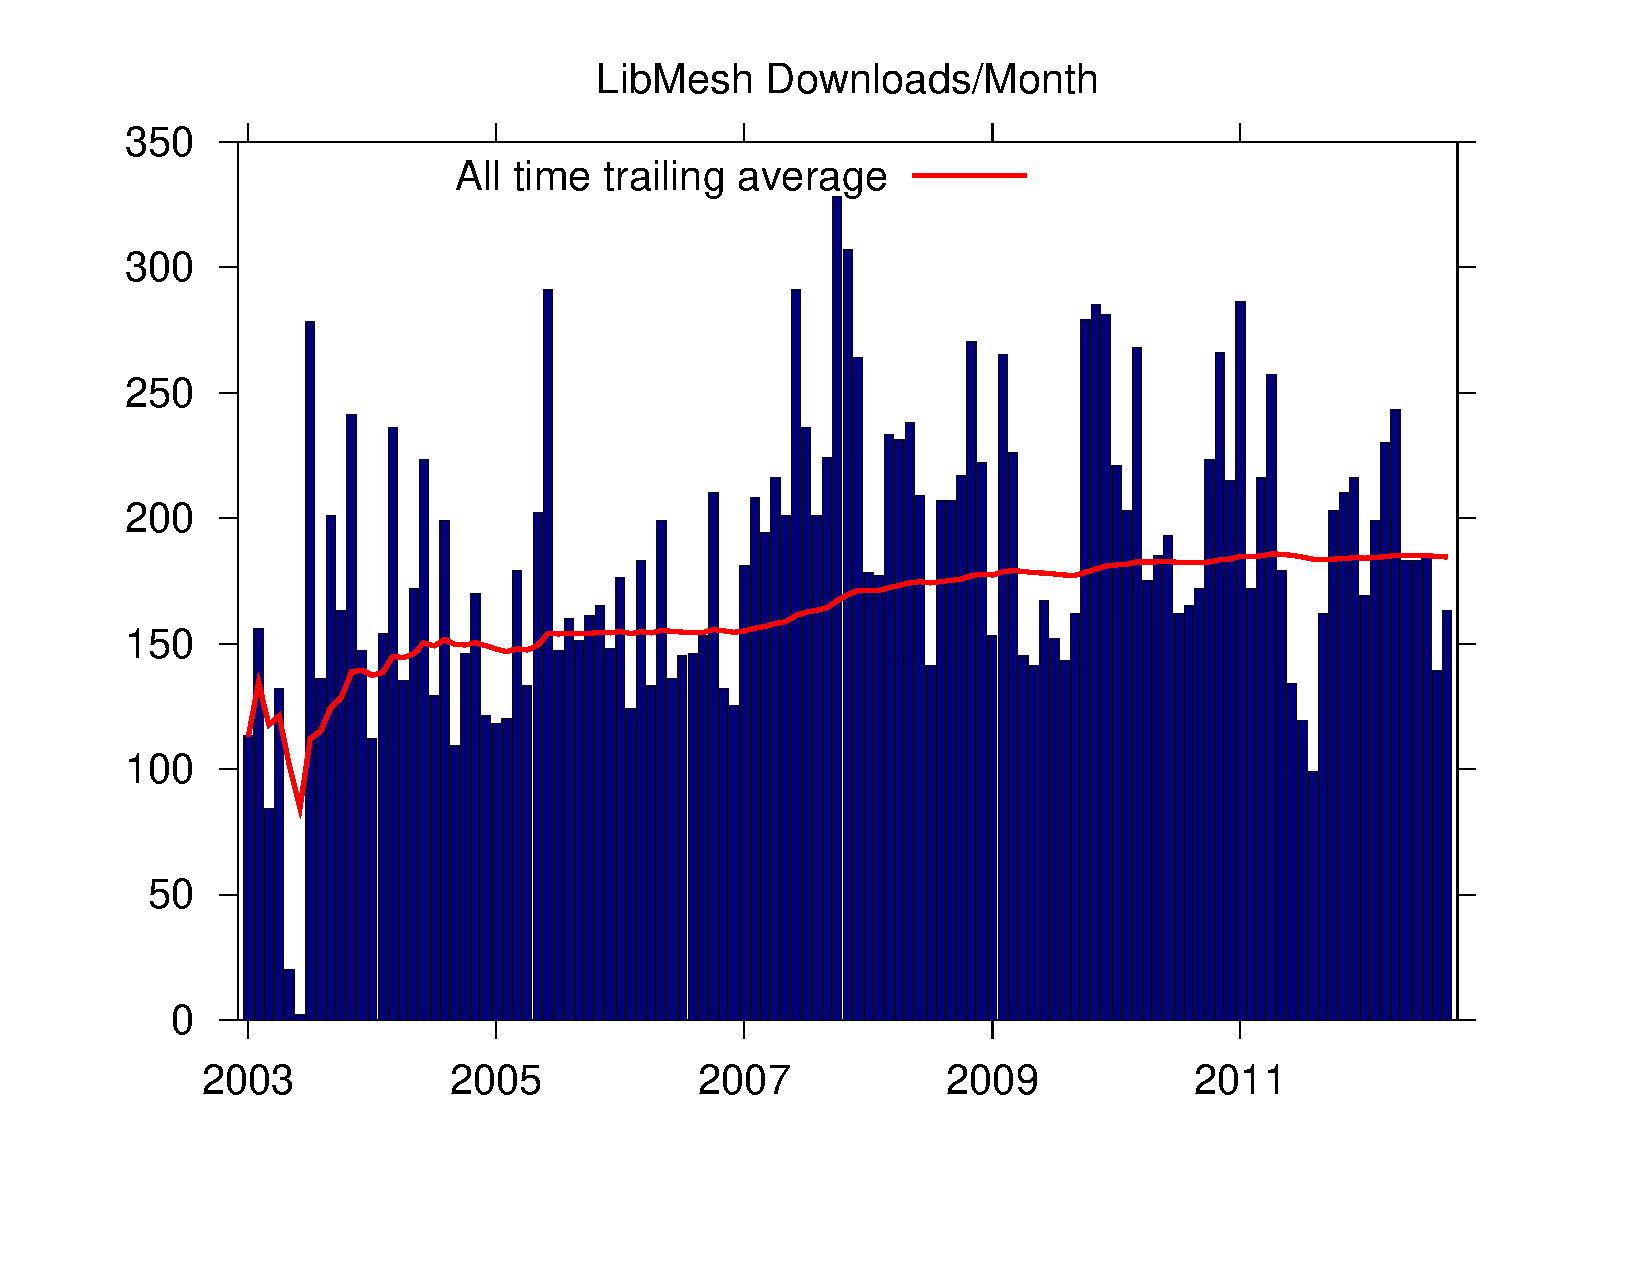
\includegraphics[viewport=55 50 760 560,
    clip=true,width=.95\textwidth]{figures/libmesh_downloads}
  %}
   % 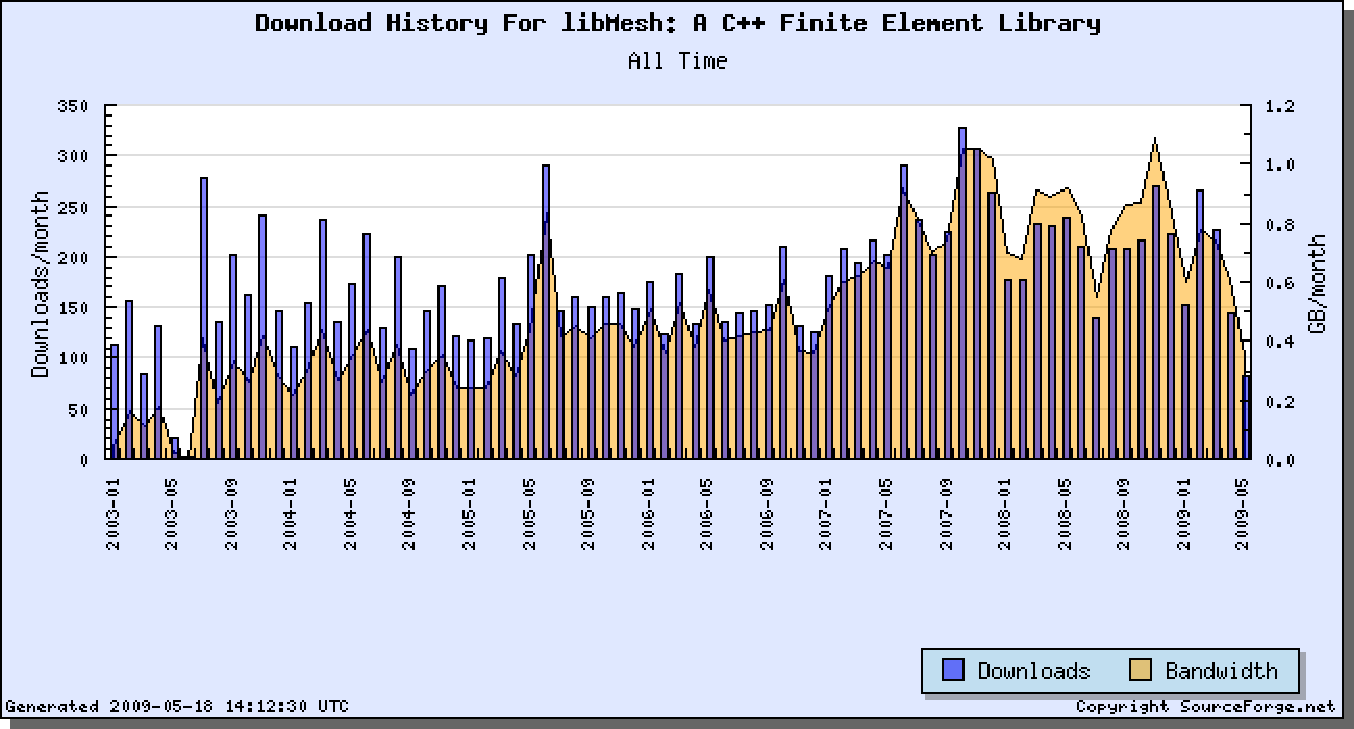
\includegraphics[width=1\textwidth]{figures/alltime_downloads}
\end{center}
%   \begin{itemize}
%   \item {Downloads/month over the life of the library.}
%   \end{itemize}
\end{frame}

\begin{frame}[t]
\begin{center}
  %\fbox{
    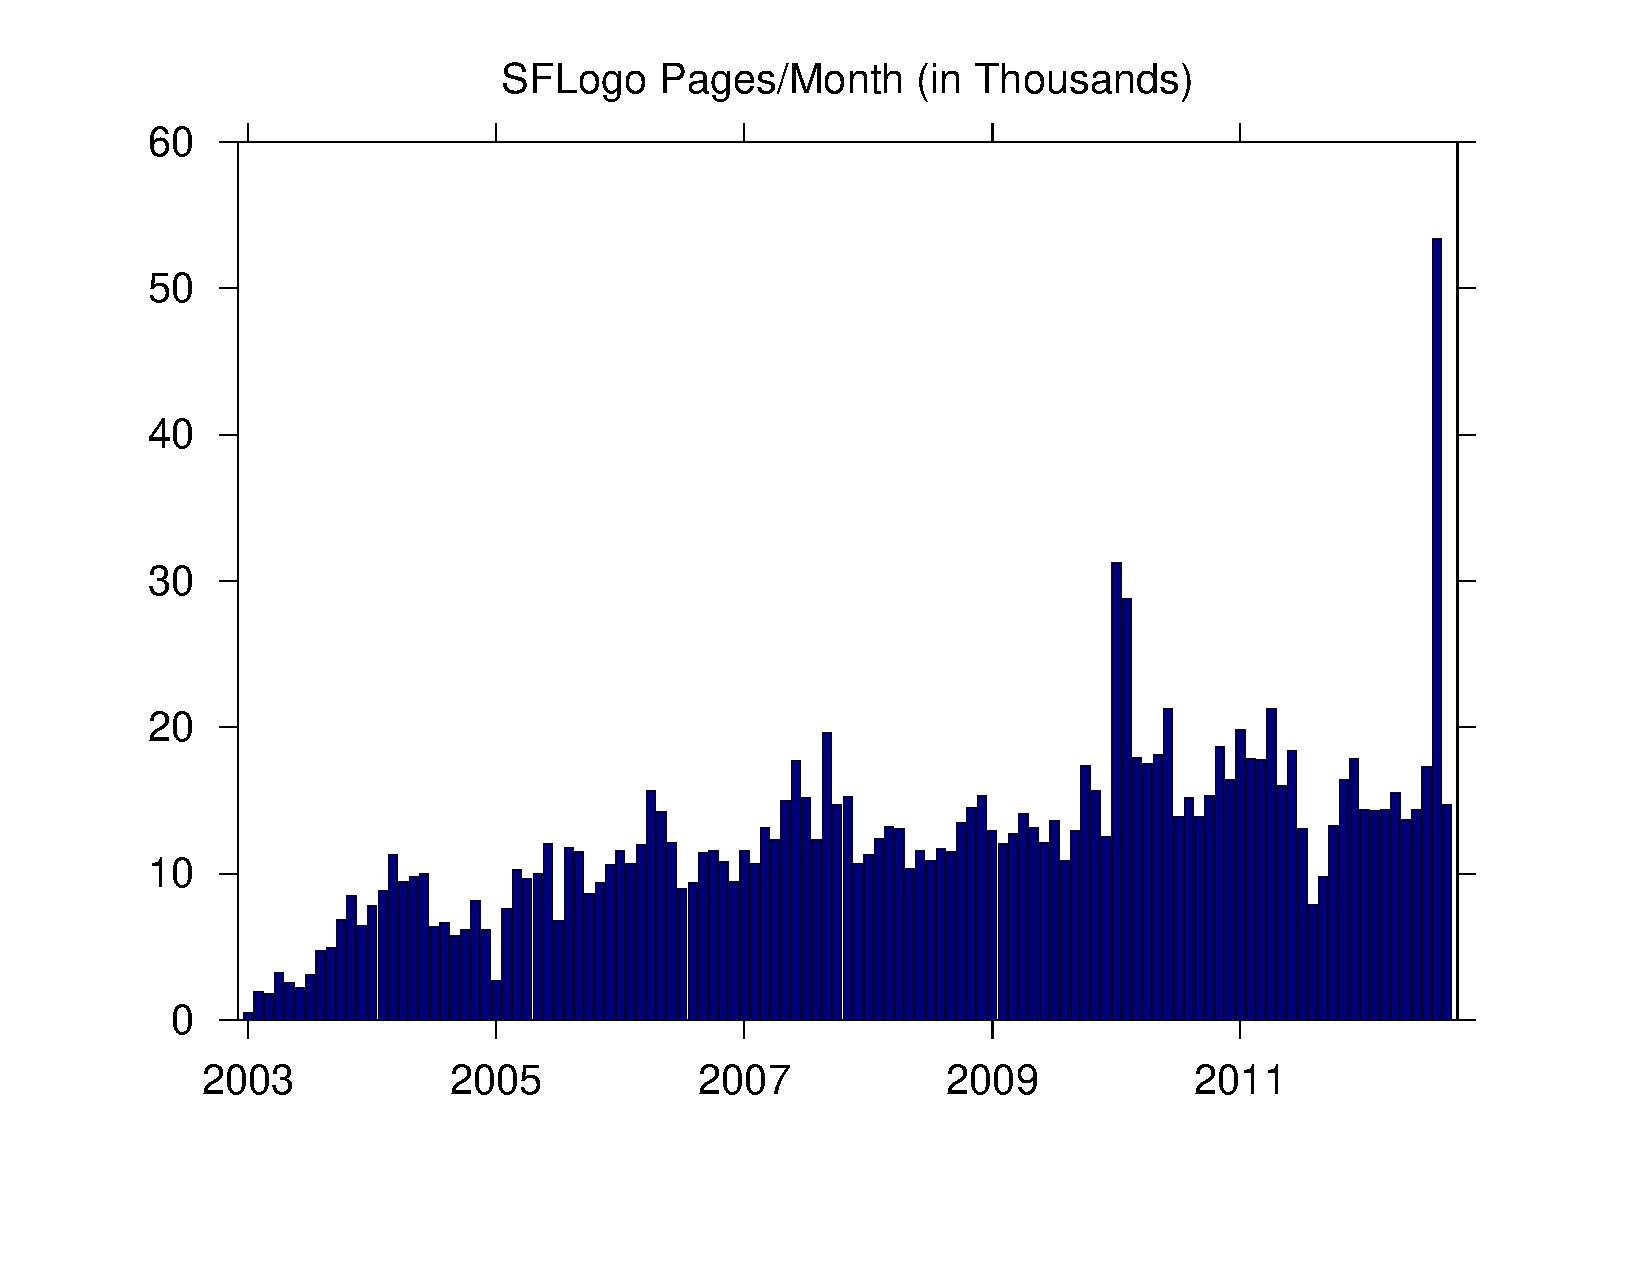
\includegraphics[viewport=55 50 760 560,
    clip=true,width=.95\textwidth]{figures/libmesh_sflogos}
  %}
   % 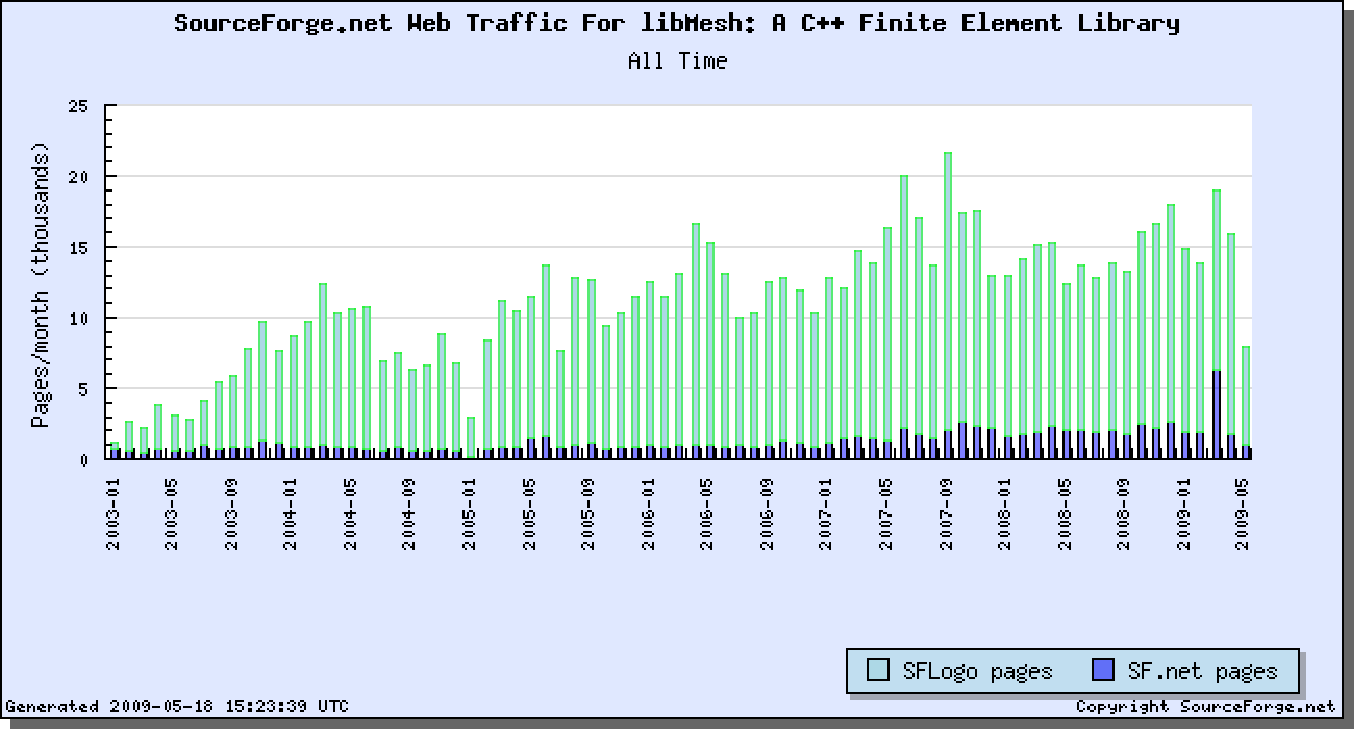
\includegraphics[width=1\textwidth]{figures/sf_web_traffic}
\end{center}
%   \begin{itemize}
%   \item {Page hits/month over the life of the library.}
%   \end{itemize}
\end{frame}



\subsection*{How big is the library?}
\begin{frame}[t]
\begin{center}
  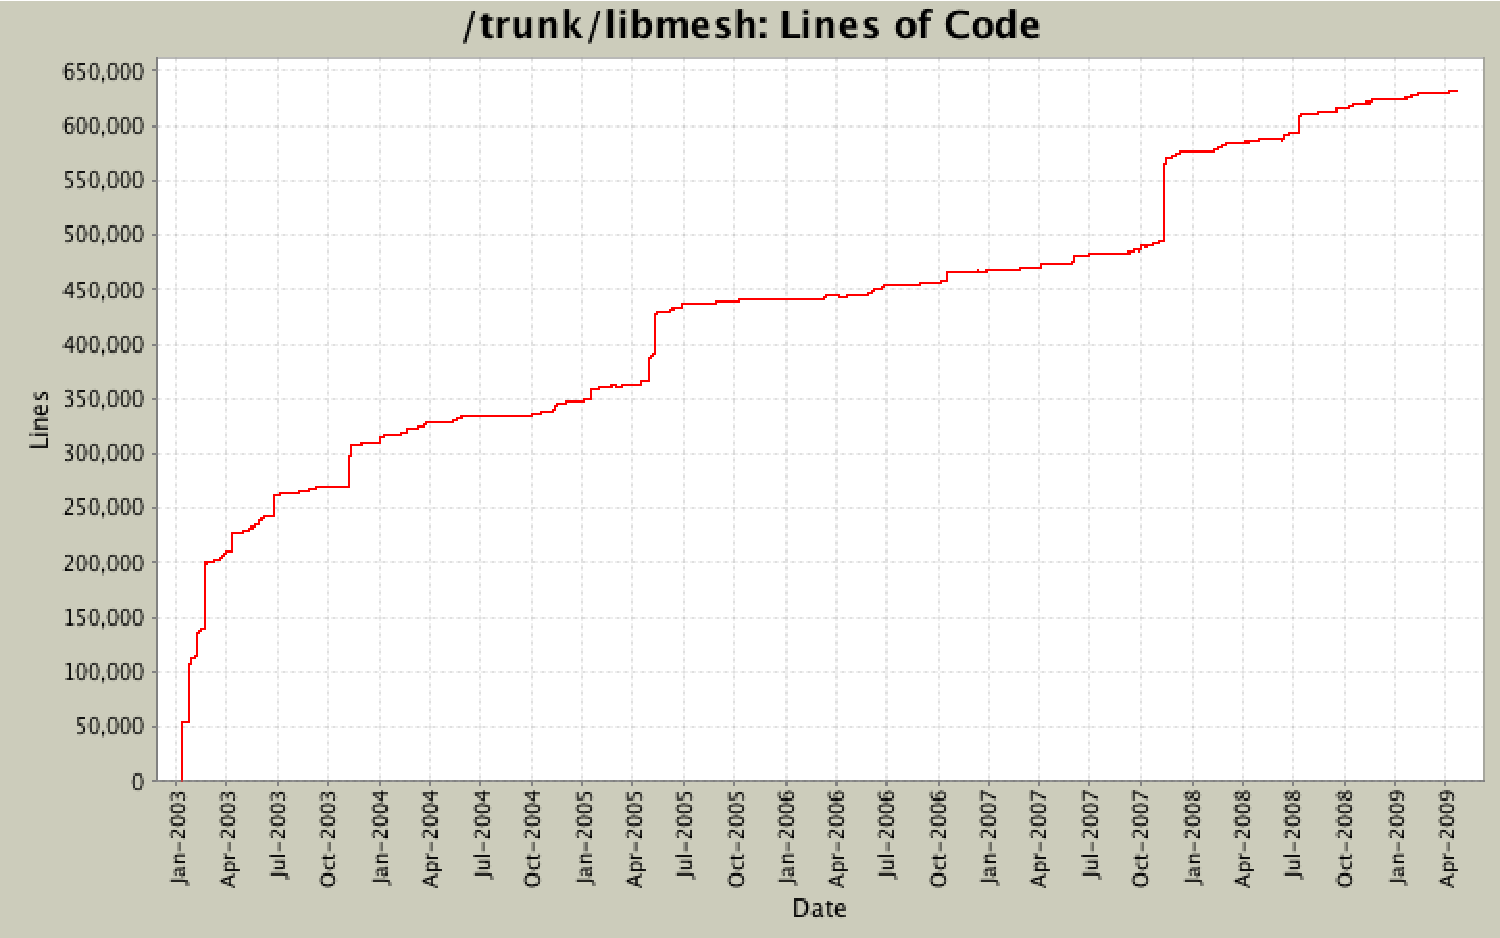
\includegraphics[width=.9\textwidth]{figures/libmesh_lines_of_code}
\end{center}
\vspace{-12pt}
  \begin{itemize}
  \item {Lines of code vs.\ time over the life of the library.}
  \end{itemize}
\end{frame}


\section{C++ and Scientific Software}
% Auto-generate the TOC slide(s)
\begin{frame}
  \tableofcontents[currentsection]
  %\tableofcontents
\end{frame}


\begin{frame}[t]
  \begin{itemize}
    \itemsep=.75cm
  \item {Wait, this is supposed to be ``Scientific Software.'' Isn't OO code `slow'?
  \only<2->
  {
    \begin{center}
      \large\alert{Yes!}
    \end{center}
  }
}
  \item<3-> {But, this is like asking if driving a car is `dangerous'.}
  \item<4-> {It is dangerous, but it is also a very convenient and effective means of transportation.}
  \item<5-> {As long as everyone plays by the rules, nobody gets hurt!}
  \end{itemize}
\end{frame}

\subsection*{Example 1: Raw vector vs.\ object }
\begin{frame}[fragile]% Must use fragile with semiverbatim!!
  \begin{itemize}
  \item {Consider a simple example using a vector to implement row-major storage.}
  \end{itemize}
\small
\begin{semiverbatim}
long matrix_size = 10000;
std::vector<double> v(matrix_size*matrix_size);

long cnt=0;
for (int i=0; i<matrix_size; ++i)
  for (int j=0; j<matrix_size; ++j)
    v[\alert<2>{i*matrix_size+j}] = cnt++;
\end{semiverbatim}
\end{frame}


\begin{frame}[fragile]% Must use fragile with semiverbatim!!
  \begin{itemize}
  \item {We can instead hide the index calculation in a user-defined Matrix type.}
  \end{itemize}
\small
\begin{semiverbatim}
class Matrix
\{
public:
  Matrix(int mm, int nn);
  double\& operator()(int i, int j);
private:
  int m, n;
  std::vector<double> vals;
\};
\end{semiverbatim}
\end{frame}


\begin{frame}[fragile]% Must use fragile with semiverbatim!!
  \begin{itemize}
  \item {The user code is now:}
  \end{itemize}
\small
\begin{semiverbatim}
long matrix_size = 10000;
Matrix m(matrix_size,matrix_size);

long cnt=0;
for (int i=0; i<matrix_size; ++i)
  for (int j=0; j<matrix_size; ++j)
    m(i,j) = cnt++;
\end{semiverbatim}
\end{frame}


\begin{frame}
  \begin{itemize}
  \item Timing results (in seconds, averaged over 5 runs) for the two different versions
    with different optimization levels.
  \end{itemize}
  \begin{center}
  \begin{tabular}{lll} \toprule
                     & \textbf{None} & \textbf{--O3} \\ \midrule
    \textbf{std::vector}  & 5.44 & 1.72  \\ 
    \textbf{Matrix}       & 6.10 & 1.70  \\ \bottomrule
  \end{tabular}
  \end{center}
\end{frame}



\begin{frame}
  \begin{itemize}
    \itemsep=1cm
  \item {With a decent compiler (in this case, \texttt{g++}) there is
      almost no difference in performance between the two.}
  \item{Does not require much advanced optimization knowledge on
      the part of the user (e.g.\ expression templates).}
  \item{The ``object'' code is arguably cleaner, and provides better
    reuse possibilities.}
  \end{itemize}
\end{frame}



\subsection*{Example 2: Virtual functions}

\begin{frame}[fragile]
  \begin{itemize}
  \item {Virtual functions are another OO feature frequently cited as ``slow.''}
  \item {Consider our previous Matrix class modified to allow subclassing:}
  \end{itemize}
\small
\begin{semiverbatim}
class MatrixBase
\{
public:
  MatrixBase(int mm, int nn);
  virtual ~MatrixBase() \{\}
  \alert{virtual} double& operator()(int i, int j) = 0;
protected:
  int m, n;
  std::vector<double> vals;
\};
\end{semiverbatim}
\end{frame}



\begin{frame}[fragile]
  \begin{itemize}
  \item {Define the MatrixRowMajor subclass to implement row-major storage:}
    % Might also want to include virtual dtor...?
    % virtual ~MatrixRowMajor() \{\}
  \end{itemize}
  \begin{semiverbatim}
\small
class MatrixRowMajor : public MatrixBase
\{
public:
  MatrixRowMajor(int mm, int nn);
  virtual double\& operator()(int i, int j);
\};

double\& MatrixRowMajor::operator()(int i, int j)
\{
  return vals[i*n + j]; \alert{// row major}
\}
  \end{semiverbatim}
\end{frame}



\begin{frame}[fragile]
  \begin{itemize}
  \item {Define the MatrixColMajor subclass for column-major storage:}
  \end{itemize}
\small
\begin{semiverbatim}
class MatrixColMajor : public MatrixBase
\{
public:
  MatrixColMajor(int mm, int nn);
  virtual double\& operator()(int i, int j);
\};

double\& MatrixColMajor::operator()(int i, int j)
\{
  return vals[i + m*j]; \alert{// col major}
\}
  \end{semiverbatim}
\end{frame}



%// ... Or, create col-major matrix
%MatrixBase\& m = *(new MatrixColMajor(matrix_size,matrix_size));

\begin{frame}[fragile]
  \begin{itemize}
  \item {(Essentially) the same matrix-fill code can be re-used...}
  \end{itemize}
\small
  \begin{semiverbatim}
// Create row-major (or col) matrix...
MatrixBase\& m = 
  *(new MatrixRowMajor(matrix_size,matrix_size));

long cnt=0;
for (int i=0; i<matrix_size; ++i)
  for (int j=0; j<matrix_size; ++j)
    m(i,j) = cnt++;
  \end{semiverbatim}
\end{frame}


\begin{frame}
  \begin{itemize}
  \item Average timing results (in seconds) for the original and
    polymorphic Matrix classes.
  \end{itemize}
  \begin{center}
  \begin{tabular}{lll} \toprule
                     & \textbf{None} & \textbf{--O3} \\ \midrule
    \textbf{Matrix}                 & 6.10 & 1.70  \\ 
    \textbf{Matrix (virtual, row-major) }       & 6.08 & 1.98  \\ 
    \textbf{Matrix (virtual, col-major) }       & 8.06 & 3.77  \\ \bottomrule

  \end{tabular}
  \end{center}
\end{frame}

\begin{frame}
  \begin{itemize}
    \itemsep=1cm
  \item {The additional flexibility obtained by decoupling the storage
      layout from the algorithm cost us about 15\% in the row-major case.}

  \item {Also, the ``generic'' algorithm (which is inherently 
      row-major) did not perform nearly as well on the column-major
      layout.}

%  \item {There are several possible solutions to this problem.}
%       \begin{enumerate}
%       \item Rework the design so that virtual functions do not appear inside
%         inner loops.
% \item Work with objects of known type (defeats purpose of polymorphism)
%       \end{enumerate}

    \item {We can address both these issues by becoming virtual at a ``higher level.''}
  \end{itemize}
\end{frame}



\begin{frame}[fragile]
  \begin{itemize}
    \itemsep=1cm
  \item {Recognizing that the algorithm is not efficiently decoupled from
      the storage layout, we can make the \emph{algorithm itself} virtual instead.}
  \end{itemize}
\small
  \begin{semiverbatim}
class MatrixBase
\{
public:
  MatrixBase(int mm, int nn);
  virtual ~MatrixBase() \{\}
  \alert{virtual void fill() = 0;}
protected:
  int m, n;
  std::vector<double> vals;
\};
\end{semiverbatim}
\end{frame}


\begin{frame}[fragile]
  \begin{itemize}
  \item {Implemented for the row-major case (col-major case
      is analogous):}
  \end{itemize}
\small
\begin{semiverbatim}
void MatrixRowMajor::fill()
\{
  long cnt=0;
  for (int i=0; i<m; ++i)
    for (int j=0; j<n; ++j)
      vals[i*n + j] = cnt++;
\}
\end{semiverbatim}
\end{frame}


\begin{frame}[fragile]
  \begin{itemize}
  \item {And finally, called generically from user code:}
  \end{itemize}
\small
  \begin{semiverbatim}
MatrixBase* m = 
  new MatrixRowMajor(matrix_size,matrix_size);
m->fill();
  \end{semiverbatim}
\end{frame}





\begin{frame}
  \begin{itemize}
  \item {Combined results for the original, non-virtual objects and the
      virtual \texttt{fill()} function.}
  \end{itemize}
  \begin{center}
  \begin{tabular}{lll} \toprule
                     & \textbf{None} & \textbf{--O3} \\ \midrule
    \textbf{std::vector}            & 5.44 & 1.72  \\ 
    \textbf{Matrix}                 & 6.10 & 1.70  \\ 
    \textbf{fill(), row-major }     & 5.70 & 1.68  \\ 
    \textbf{fill(), col-major }     & 5.71 & 1.69  \\ \bottomrule
  \end{tabular}
  \end{center}
\end{frame}


\begin{frame}
  \begin{itemize}
    \itemsep=.65cm
  \item {Proper use of virtual functions (i.e.\ not too many) leads to
    more flexible code with the same performance as less flexible code.}

  \item {The \texttt{fill()} method in this example can be made more sophisticated
      if we also pass a ``\texttt{Filler}'' function object to it. }

  \item {This example was trivial: there are libraries
      (boost/blitz/eigen) which are much more realistic.}

  \item{The guidelines developed here for using virtual functions should
    apply in other situations as well.}

  \end{itemize}
\end{frame}

% LocalWords:  LibMesh LGPL multi CFDLab TACC Stogner advisor Dreyer TUHH INL
% LocalWords:  Knezevic ger Universit Coutinho Certik thi Ruijter Mahadevan OO
% LocalWords:  Garg libmesh cnt nn vals lll subclassing MatrixBase
% LocalWords:  MatrixRowMajor MatrixColMajor



\end{document}

% LocalWords:  LibMesh LGPL multi CFDLab TACC Stogner advisor Dreyer TUHH INL
% LocalWords:  Knezevic ger Universit Coutinho Certik thi Ruijter Mahadevan OO
% LocalWords:  Garg libmesh cnt nn vals lll subclassing MatrixBase rayleigh
% LocalWords:  MatrixRowMajor MatrixColMajor cpp poisson discretized
